\documentclass[12pt,]{article}
\usepackage{lmodern}
\usepackage{amssymb,amsmath}
\usepackage{ifxetex,ifluatex}
\usepackage{fixltx2e} % provides \textsubscript
\ifnum 0\ifxetex 1\fi\ifluatex 1\fi=0 % if pdftex
  \usepackage[T1]{fontenc}
  \usepackage[utf8]{inputenc}
\else % if luatex or xelatex
  \ifxetex
    \usepackage{mathspec}
  \else
    \usepackage{fontspec}
  \fi
  \defaultfontfeatures{Ligatures=TeX,Scale=MatchLowercase}
\fi
% use upquote if available, for straight quotes in verbatim environments
\IfFileExists{upquote.sty}{\usepackage{upquote}}{}
% use microtype if available
\IfFileExists{microtype.sty}{%
\usepackage{microtype}
\UseMicrotypeSet[protrusion]{basicmath} % disable protrusion for tt fonts
}{}
\usepackage[margin=1in]{geometry}
\usepackage{hyperref}
\PassOptionsToPackage{usenames,dvipsnames}{color} % color is loaded by hyperref
\hypersetup{unicode=true,
            pdftitle={Which Stats Method?},
            pdfauthor={Richard White},
            colorlinks=true,
            linkcolor=Maroon,
            citecolor=Blue,
            urlcolor=Blue,
            breaklinks=true}
\urlstyle{same}  % don't use monospace font for urls
\usepackage{natbib}
\bibliographystyle{apalike}
\usepackage{longtable,booktabs}
\usepackage{graphicx,grffile}
\makeatletter
\def\maxwidth{\ifdim\Gin@nat@width>\linewidth\linewidth\else\Gin@nat@width\fi}
\def\maxheight{\ifdim\Gin@nat@height>\textheight\textheight\else\Gin@nat@height\fi}
\makeatother
% Scale images if necessary, so that they will not overflow the page
% margins by default, and it is still possible to overwrite the defaults
% using explicit options in \includegraphics[width, height, ...]{}
\setkeys{Gin}{width=\maxwidth,height=\maxheight,keepaspectratio}
\IfFileExists{parskip.sty}{%
\usepackage{parskip}
}{% else
\setlength{\parindent}{0pt}
\setlength{\parskip}{6pt plus 2pt minus 1pt}
}
\setlength{\emergencystretch}{3em}  % prevent overfull lines
\providecommand{\tightlist}{%
  \setlength{\itemsep}{0pt}\setlength{\parskip}{0pt}}
\setcounter{secnumdepth}{5}
% Redefines (sub)paragraphs to behave more like sections
\ifx\paragraph\undefined\else
\let\oldparagraph\paragraph
\renewcommand{\paragraph}[1]{\oldparagraph{#1}\mbox{}}
\fi
\ifx\subparagraph\undefined\else
\let\oldsubparagraph\subparagraph
\renewcommand{\subparagraph}[1]{\oldsubparagraph{#1}\mbox{}}
\fi

%%% Use protect on footnotes to avoid problems with footnotes in titles
\let\rmarkdownfootnote\footnote%
\def\footnote{\protect\rmarkdownfootnote}

%%% Change title format to be more compact
\usepackage{titling}

% Create subtitle command for use in maketitle
\newcommand{\subtitle}[1]{
  \posttitle{
    \begin{center}\large#1\end{center}
    }
}

\setlength{\droptitle}{-2em}

  \title{Which Stats Method?}
    \pretitle{\vspace{\droptitle}\centering\huge}
  \posttitle{\par}
    \author{Richard White}
    \preauthor{\centering\large\emph}
  \postauthor{\par}
      \predate{\centering\large\emph}
  \postdate{\par}
    \date{2018-11-01}

\usepackage{booktabs}

\begin{document}
\maketitle

{
\hypersetup{linkcolor=black}
\setcounter{tocdepth}{2}
\tableofcontents
}
\listoftables
\listoffigures
\section*{Syllabus}\label{syllabus}
\addcontentsline{toc}{section}{Syllabus}

\textbf{Instructor:} Richard White
{[}\href{mailto:richard.white@fhi.no}{\nolinkurl{richard.white@fhi.no}}{]}

\textbf{Time:} 09:00 - 11:45, 18th September 2017

\textbf{Location:} Main auditorium, L8, Lindern Campus,
Folkehelseinstittutet, Oslo

\textbf{Language:} English

\textbf{Format and Procedures}

09:00 - 10:00: Lecture 1

10:00 - 10:10: Break

10:10 - 11:10: Lecture 2

10:10 - 10:15: Break

11:15 - 11:45: Examples from FHI

\textbf{Description}

This course will provide a basic overview of general statistical
methodology that can be useful in the areas of infectious diseases,
environmental medicine, and labwork. By the end of this course, students
will be able to identify appropriate statistical methods for a variety
of circumstances.

This course will \textbf{not} teach students how to implement these
statistical methods, as there is not sufficient time. The aim of this
course is to enable the student to identify which methods are required
for their study, allowing the student to identify their needs for
subsequent methods courses, self-learning, or external help.

You should register for this course if you are one of the following:

\begin{itemize}
\tightlist
\item
  Have experience with applying statistical methods, but are sometimes
  confused or uncertain as to whether or not you have selected the
  correct method.
\item
  Do not have experience with applying statistical methods, and would
  like to get an overview over which methods are applicable for your
  projects so that you can then undertake further studies in these
  areas.
\end{itemize}

\textbf{Lecture 1}

\begin{enumerate}
\def\labelenumi{\arabic{enumi}.}
\tightlist
\item
  Identifying continuous, categorical, count, and censored variables
\item
  Identifying exposure and outcome variables
\item
  Identifying when t-tests (paired and unpaired) should be used
\item
  Identifying when non-parametric t-test equivalents should be used
\item
  Identifying when ANOVA should be used
\item
  Identifying when linear regression should be used
\item
  Identifying the similarities between t-tests, ANOVA, and regression
\item
  Identifying when logistic regression models should be used
\item
  Identifying when Poisson/negative binomial and cox regression models
  should be used
\item
  Identifying when chi-squared/fisher's exact test should be used
\end{enumerate}

\textbf{Lecture 2}

\begin{enumerate}
\def\labelenumi{\arabic{enumi}.}
\tightlist
\item
  Identifying when data does not have any dependencies (i.e.~all
  observations are independent of each other) versus when data has
  complicated dependencies (i.e.~longitudinal data, matched data,
  multiple cohorts)
\item
  Identifying when mixed effects regression models should be used
\item
  Identifying when conditional logistic regression models should be used
\item
  (TBD) Understanding the different imputation methods used when lab
  data is below the limit of detection (LOD)
\item
  (TBD) Understanding the best practices for data files and project
  folders
\end{enumerate}

\textbf{Prerequisites}

To participate in this course it is recommended that you have some
experience with either research or data.

\textbf{Additional information}

For the last 30 minutes of the course we will be going through examples
of analyses performed at FHI and identifying which statistical methods
are appropriate. If you would like your analysis to be featured/included
in this section, please send an email to
\href{mailto:richard.white@fhi.no}{\nolinkurl{richard.white@fhi.no}}
briefly describing your problem.

\section{Reference}\label{reference}

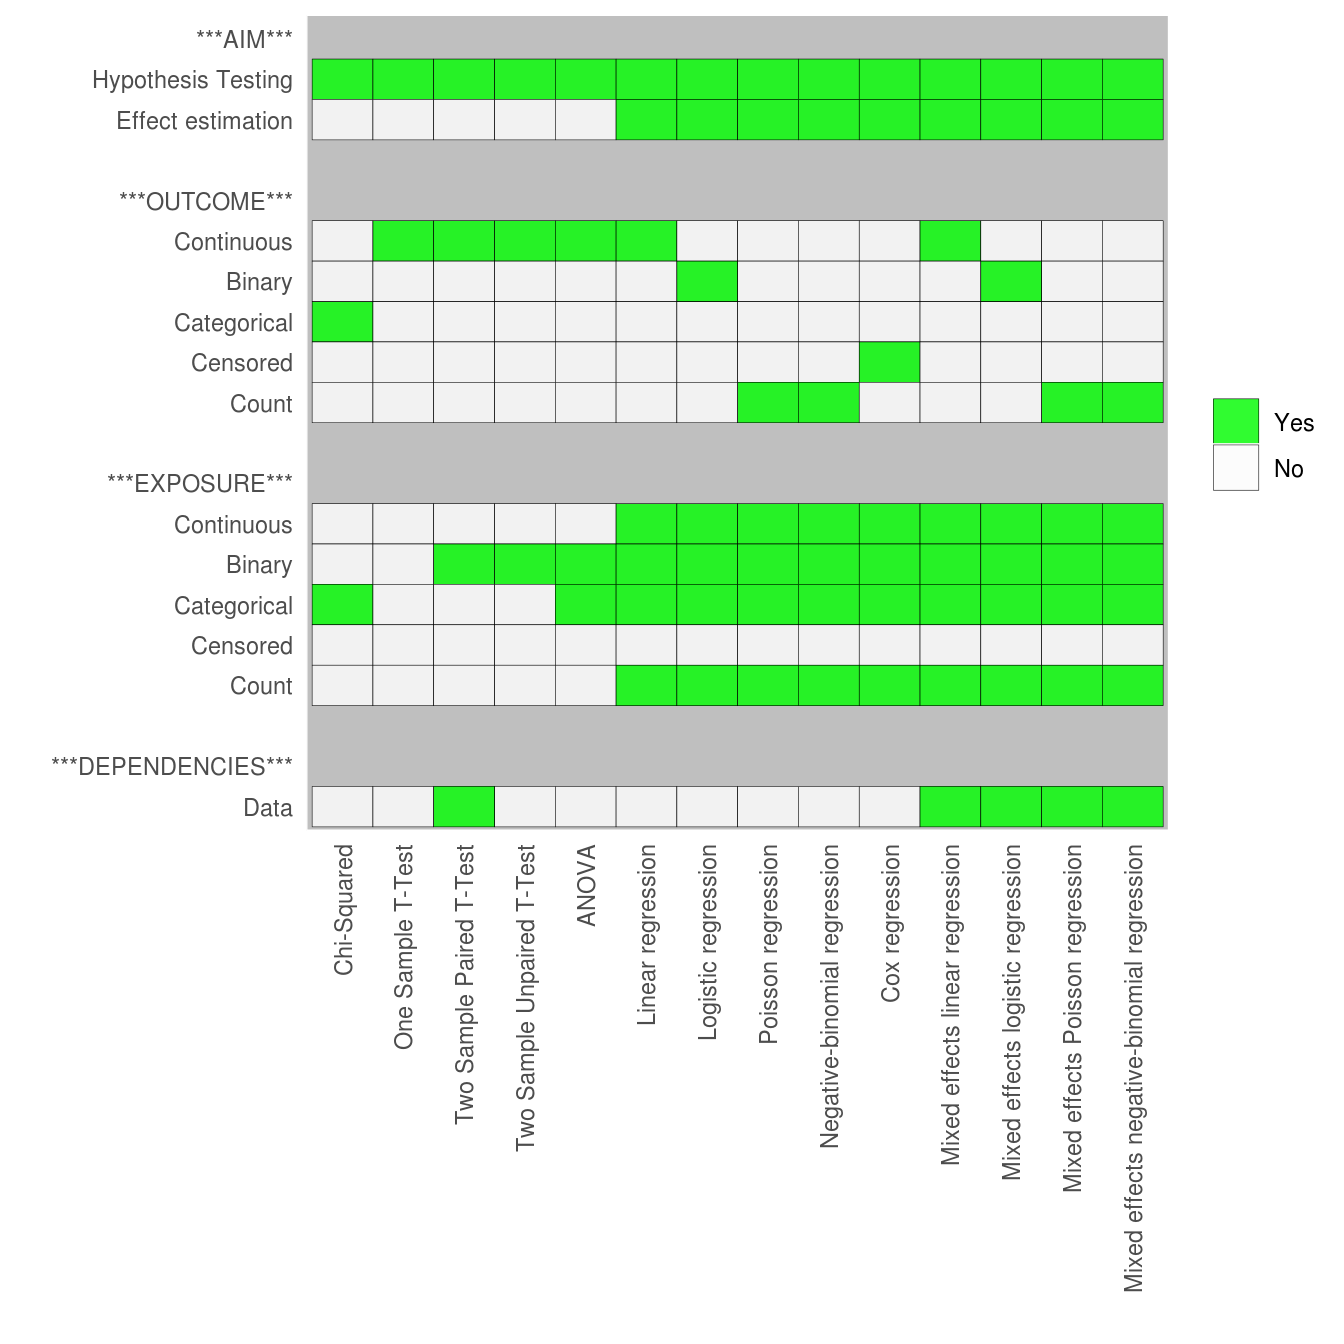
\includegraphics{website_files/figure-latex/unnamed-chunk-1-1.pdf}

\section{Variables}\label{variables}

\subsection{Introduction}\label{introduction}

A variable is anything that can be measured or counted. In general, we
think of our datasets as a rectangle, with a column for each variable
and a row for each observation (there are some exceptions when
discussing long/wide formatted data, but that is out of the scope of
this course).

We care about four attributes of the variables:

\begin{itemize}
\tightlist
\item
  the variable's type (statistical relevance)
\item
  the different values the variable can take (statistical relevance)
\item
  is the variable clean (i.e.~ready to use in an analysis?) (statistical
  relevance)
\item
  the name of the variable (useful for us)
\end{itemize}

We can use the fourth attribute to help us remember the first three.

\subsection{Continuous Variables}\label{continuous-variables}

A variable is continuous there is a meaningful ``distance'' between
values.

For example:

\begin{itemize}
\tightlist
\item
  Temperature
\item
  Weight
\item
  Height
\item
  BMI
\item
  Blood pressure
\item
  \hfill \break
  \hfill \break
\item
  \hfill \break
  \hfill \break
\end{itemize}

Clean continuous variables can be given the prefix \texttt{con\_} to
denote that they are clean. For example, \texttt{temperature} could be
called \texttt{con\_temperature} after it has been cleaned and is ready
for analysis.

\subsection{Binary Variables}\label{binary-variables}

A variable is binary if it can only hold two values.

For example:

\begin{itemize}
\tightlist
\item
  0 or 1
\item
  True or false
\item
  Male or female
\item
  Sick or healthy
\item
  Born in Norway vs Born outside of Norway
\item
  \hfill \break
  \hfill \break
\item
  \hfill \break
  \hfill \break
\end{itemize}

Clean binary variables can be given the prefix \texttt{is\_} to denote
that they are clean, binary, and reference the ``active state''. For
example, an unclean variable called \texttt{sex} could be recoded as 0
for female and 1 for male, then called \texttt{is\_male} to denote that
it is clean (ready for analysis), binary, and ``male'' is the active
state when \texttt{is\_male=1}.

\subsection{Categorical Variable}\label{categorical-variable}

A variable is categorical if there is no meaningful ``distance'' between
values.

For example:

\begin{itemize}
\tightlist
\item
  Sick or healthy
\item
  Born in Norway vs Born outside of Norway
\item
  Cancer stage (I, II, III, or IV)
\item
  BMI category (underweight, normal, or overweight)
\item
  \hfill \break
  \hfill \break
\item
  \hfill \break
  \hfill \break
\end{itemize}

Clean categorical variables can be given the prefix \texttt{cat\_} to
denote that they are clean. For example, \texttt{BMI\ category} could be
called \texttt{cat\_bmi} after it has been cleaned and is ready for
analysis.

\subsection{Censored Variables}\label{censored-variables}

Censored variables are a subset of continuous variables. They are
artificially cutoff (``censored'') at some point.

For example:

\begin{itemize}
\tightlist
\item
  Height -- if everyone over 175cm is recorded as ``175+''
\item
  Age -- if everyone under 10 years old is recorded as
  ``\textless{}=10''
\item
  Time alive since receiving illness diagnosis if there is loss to
  followup (i.e.~we know that the person has lived at least 4 years
  before we lost track of them)
\item
  \hfill \break
  \hfill \break
\item
  \hfill \break
  \hfill \break
\end{itemize}

Clean censored variables can be given the prefix \texttt{cen\_} to
denote that they are clean. For example,
\texttt{time\ alive\ since\ receiving\ illness\ diagnosis} could be
called \texttt{cen\_time\_alive} after it has been cleaned and is ready
for analysis.

\subsection{Count Variables}\label{count-variables}

Count variables are a subset of continuous variables. They can only have
integer values (e.g.~0, 1, 2, 3).

For example:

\begin{itemize}
\tightlist
\item
  Number of cars that use the parking lot in a day
\item
  Number of influenza patients who use the hospital every day
\item
  Number of tuberculosis patients who are screened every year
\item
  \hfill \break
  \hfill \break
\item
  \hfill \break
  \hfill \break
\end{itemize}

Clean count variables can be given the prefix \texttt{cou\_} to denote
that they are clean. For example, \texttt{number\ of\ cars} could be
called \texttt{cou\_num\_cars} after it has been cleaned and is ready
for analysis.

\subsection{Independent Versus Dependent
Variables}\label{independent-versus-dependent-variables}

An independent variable is often called an exposure or predictor
variable. In an experiment, this variable is manipulated by the
researcher.

A dependent variable is often called the outcome. In research, we
generally want to see if (the following all mean the same thing):

\begin{itemize}
\tightlist
\item
  The dependent variable is dependent on the independent variable
\item
  The predictor variable predicts the outcome.
\item
  The exposure affects the outcome
\end{itemize}

For ease of understanding, we will use the terms ``outcome'' and
``exposure'' for the rest of this course.

\subsection{Dataset workflow
(pipeline)}\label{dataset-workflow-pipeline}

\begin{itemize}
\tightlist
\item
  We begin with a raw dataset (this is never altered)
\item
  We clean the raw dataset and create new variables as needed
\item
  We save a ``clean'' dataset (all variables have the prefixes
  \texttt{c\_} or \texttt{is\_})
\item
  We ONLY run analyses on the clean dataset
\end{itemize}

We do all of this in ``do files'' that allow us to recreate the clean
dataset from the raw dataset.

Think of our analysis as making dinner, with the \texttt{do\ files} as
our \texttt{recipe} and the \texttt{raw\ dataset} as our
\texttt{raw\ ingredients}. The \texttt{recipe} tells us how to prepare
the \texttt{raw\ ingredients} (\texttt{clean\ dataset}) and how to
\texttt{cook} (\texttt{analyse}) the \texttt{prepared\ ingredients}
(\texttt{clean\ dataset}) to produce the \texttt{food}
(\texttt{results}).

All we need are \texttt{raw\ ingredients} and the \texttt{recipe}! The
\texttt{prepared\ ingredients} and the \texttt{food} are downstream
by-products!

This means that if our code is written correctly, we can delete our
\texttt{clean\ datasets} and \texttt{results} without any worry, because
the \texttt{raw\ dataset} and \texttt{do\ files} are sufficient.

\section{Simple Hypothesis Testing: Chi-Squared, T-tests, and
ANOVA}\label{simple-hypothesis-testing-chi-squared-t-tests-and-anova}

\subsection{Hypothesis Testing}\label{hypothesis-testing}

In science, we are interested in testing hypotheses. Statistics allows
us to formally test our hypotheses. In statistical testing we have a
\textbf{null} hypothesis (\(\text{H}_0\)) and an \textbf{alternative}
hypothesis (\(\text{H}_1\)). We assume the null hypothesis is true and
try to find the probability of what we have observed (or something more
extreme). If our observations are very unlikely (assuming the null
hypothesis is true) then we reject the null hypothesis in favor of the
alternative hypothesis.

For example:

\[\text{H}_0: \text{It is summer}\]
\[\text{H}_1: \text{It is not summer}\]

Our observed data for today is a maximum temperature of -20C. Assuming
it is summer, how likely is it that today's maximum temperature will be
-20C? Not very likely! We therefore reject \(\text{H}_0\) (``it is
summer'') in favor of \(\text{H}_1\) (``it is not summer''). That is, we
conclude that it is not summer today.

\subsection{Which Method To Use?}\label{which-method-to-use}

Deciding on the appropriate statistical method is (in principle) fairly
easy. You just look at the:

\begin{itemize}
\tightlist
\item
  Aim (hypothesis testing or estimation of effect size?)
\item
  Outcome type (continuous, binary, categorical, censored, count)
\item
  Exposure (type)
\item
  Parametric assumptions
\item
  Dependencies in the data
\end{itemize}

and we then (essentially) use a flowchart.

\subsection{Chi-Squared Test}\label{chi-squared-test}

A Chi-Squared test is used to test if two categorical variables are
associated with each other.

\subsubsection{Aim/Outcome/Exposure/Parametric/Dependencies}\label{aimoutcomeexposureparametricdependencies}

\textbf{Aim}: Hypothesis testing (testing if two categorical variables
are associated with each other.)

\textbf{Outcome}: Categorical variable

\textbf{Exposure}: Categorical variable

\textbf{Parametric assumptions}: No

\textbf{Dependencies}: None (all observations independent)

\subsubsection{Examples}\label{examples}

\begin{itemize}
\tightlist
\item
  Testing if people's country of origin (Norway/Not Norway) is
  associated with tuberculosis status (never had TB/has had TB)
\item
  Testing if people's region of origin (Europe/North America/South
  America/Other) is associated with marital status
  (Single/Married/Divorced)
\item
  Testing if county of residence (Oslo, Akershus, etc) is associated
  with post-surgery infection status (No infection/mild infection/deep
  infection)
\item
  \hfill \break
  \hfill \break
\item
  \hfill \break
  \hfill \break
\end{itemize}

\newpage

\subsection{One Sample T-Test}\label{one-sample-t-test}

A one sample t-test tests if the mean of a continuous variable differs
from a specified value (generally zero)

\[\text{H}_0: \mu = 180\] \[\text{H}_1: \mu \ne 180\]

Or rephrased:

\[\text{H}_0: \text{The average height of men is equal to 180cm}\]
\[\text{H}_1: \text{The average height of men is not equal to 180cm}\]

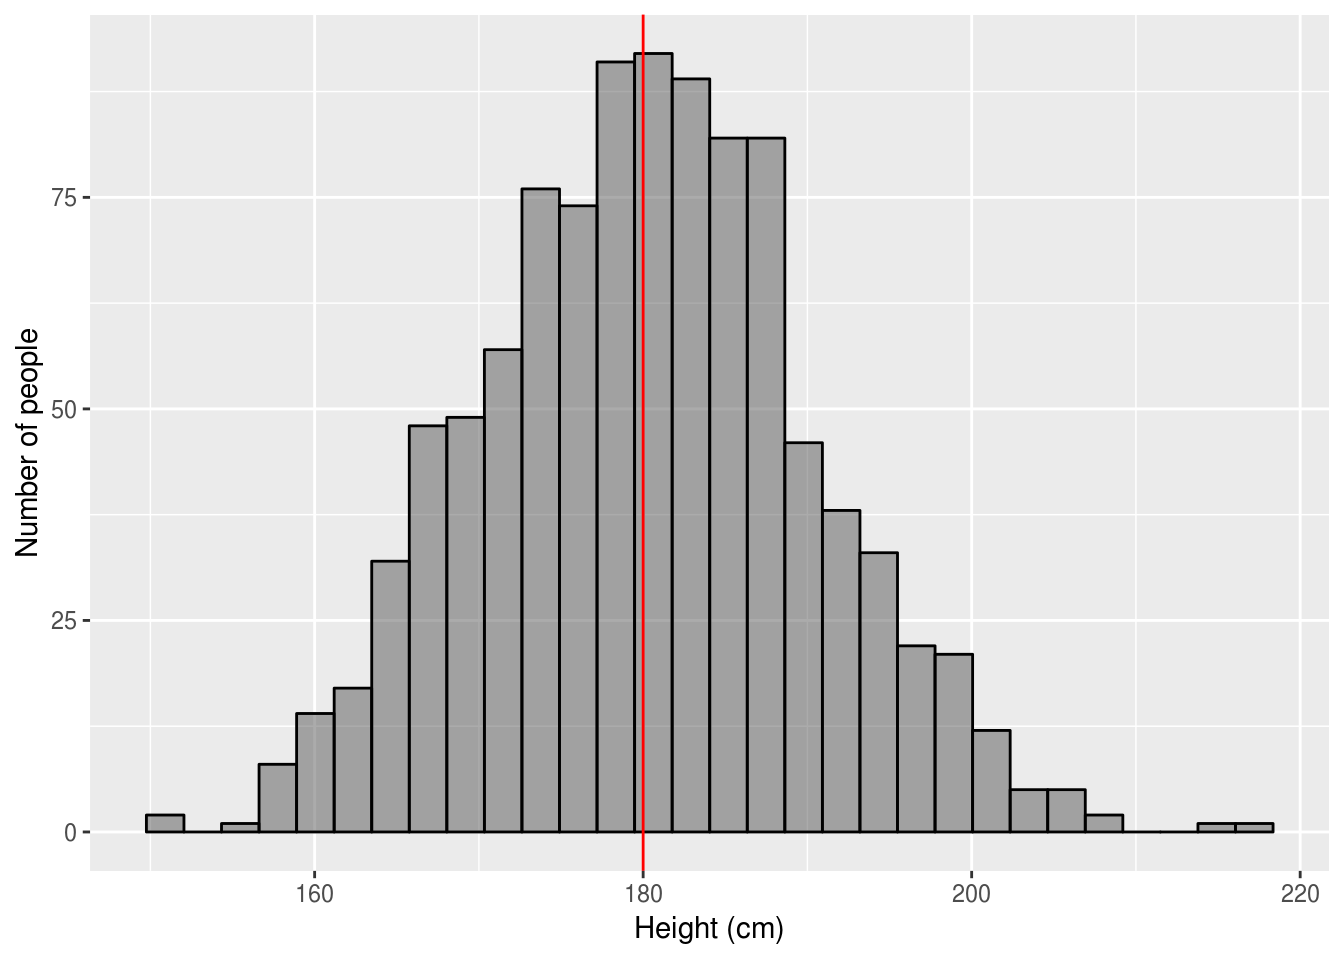
\includegraphics{website_files/figure-latex/unnamed-chunk-2-1.pdf}

\subsubsection{Aim/Outcome/Exposure/Parametric/Dependencies}\label{aimoutcomeexposureparametricdependencies-1}

\textbf{Aim}: Hypothesis testing (test if the mean of a continuous
variable differs from a specified value)

\textbf{Outcome}: Continuous variable

\textbf{Exposure}: Does not exist

\textbf{Parametric assumptions}: Outcome is distributed as a Normal
distribution

\textbf{Dependencies}: None (all observations independent)

\subsubsection{Example 1}\label{example-1}

\(\rightarrow\) Testing if the average BMI of Norwegians is equal to 23

\[H_0: \mu_{\text{bmi}} = 23\] \[H_1: \mu_{\text{bmi}} \ne 23\]

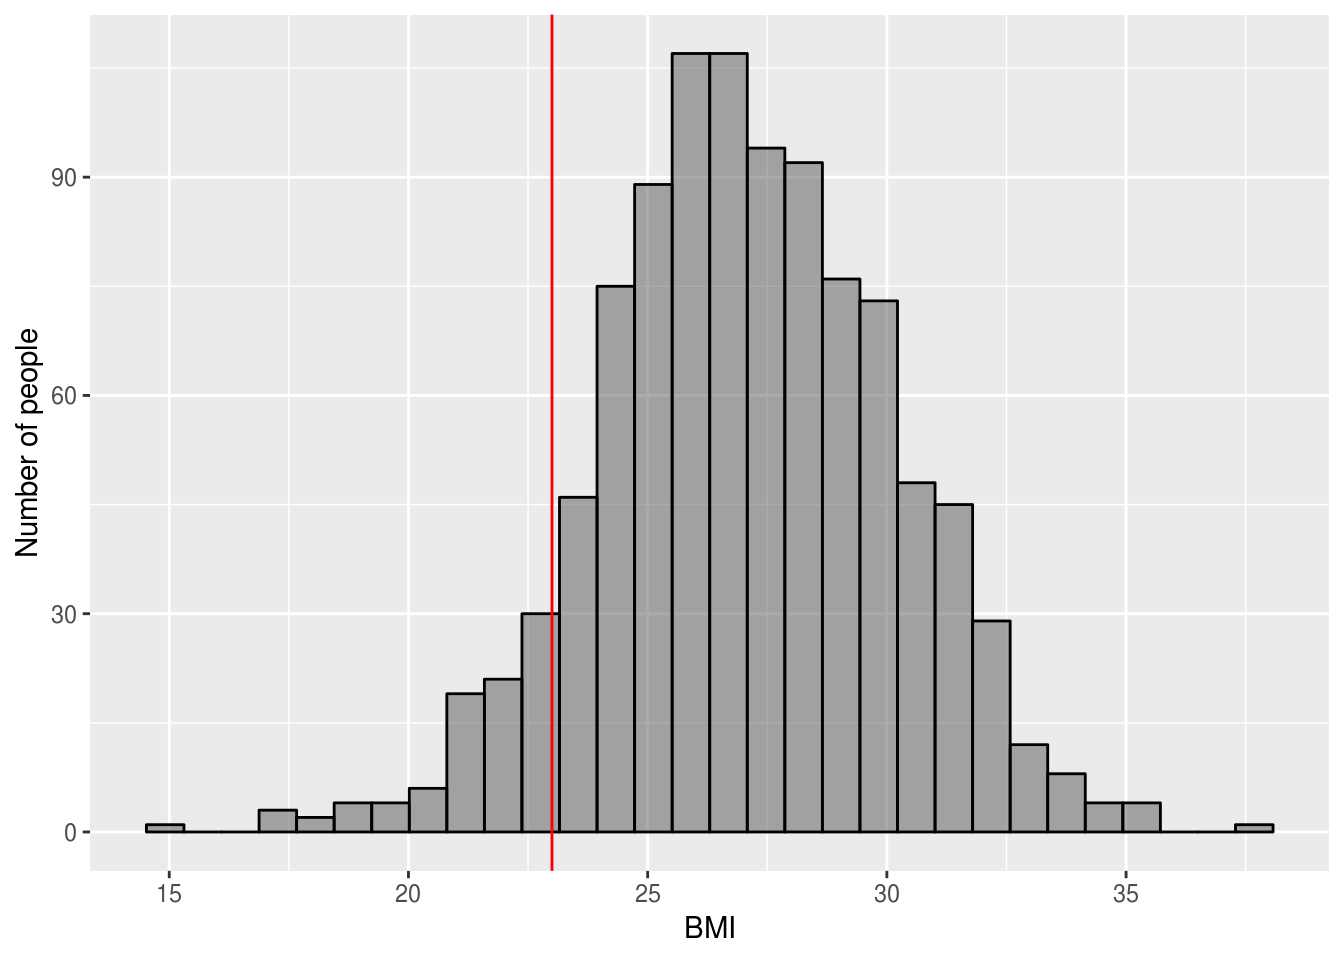
\includegraphics{website_files/figure-latex/unnamed-chunk-3-1.pdf}

\newpage

\subsubsection{Example 2}\label{example-2}

\(\rightarrow\) Testing if the average pH of tap water is equal to 7

\[H_0: \mu_{\text{pH}} = 7\] \[H_1: \mu_{\text{pH}} \ne 7\]

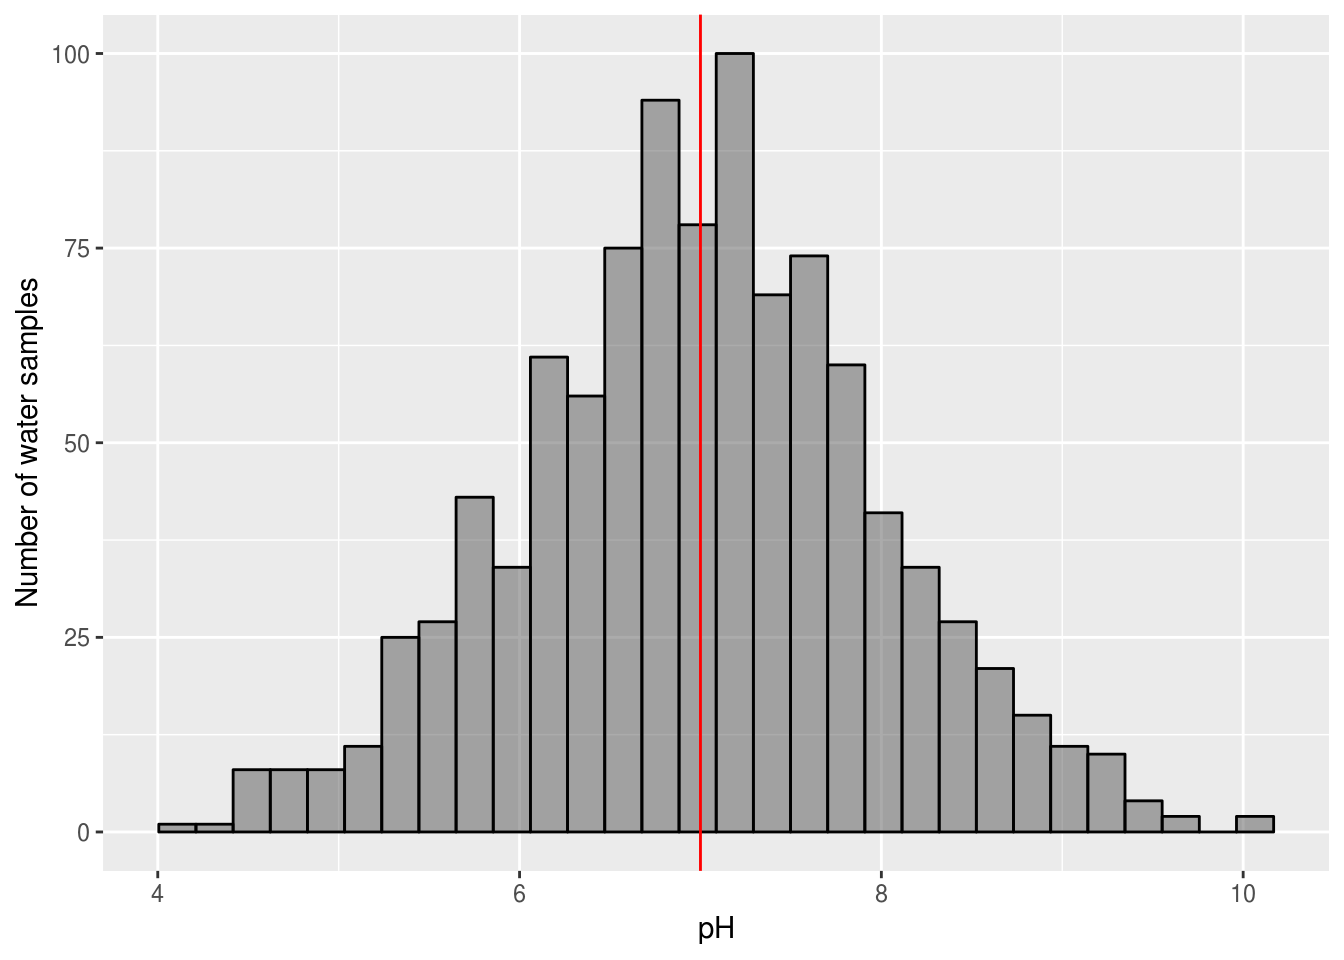
\includegraphics{website_files/figure-latex/unnamed-chunk-4-1.pdf}

\subsubsection{Example 3}\label{example-3}

\(\rightarrow\) \hfill \break
\hfill \break
\hfill \break
\(H_0:\) \hfill \break
\hfill \break
\hfill \break
\(H_1:\)

\newpage 

\subsubsection{Example 4}\label{example-4}

\(\rightarrow\) \hfill \break
\hfill \break
\hfill \break
\(H_0:\) \hfill \break
\hfill \break
\hfill \break
\(H_1:\)

\subsection{Two sample T-Tests}\label{two-sample-t-tests}

A t-test tests if the mean of a continuous variable differs between two
groups. There are two kinds of two-sample t-tests: paired and unpaired.

\subsection{Two-sample Paired T-Test}\label{two-sample-paired-t-test}

A paired t-test is a special case where we have \(N\) participants, and
each participant has two observations (generally ``before experiment''
and ``after experiment''). We want to test if the mean of outcome
variable differs between ``after'' and ``before''.

For example, in a weight-loss experiment, we have \(N\) participants and
we want to see if the average ``after weight'' is different from the
average ``before weight''.

This is done by subtracting the outcome from one group (``before
weight'') from the outcome in the other group (``after weight'') for
each person (``difference in weight''), and then performing a one-sample
t-test to see if the mean of this variable is different from zero.

\[\text{H}_0: \mu_{\text{after}-\text{before}} = 0\]
\[\text{H}_1: \mu_{\text{after}-\text{before}} \ne 0\]

\subsubsection{Aim/Outcome/Exposure/Parametric/Dependencies}\label{aimoutcomeexposureparametricdependencies-2}

\textbf{Special preprocessing of data}: for each participant subtract
the ``before'' observation from the ``after'' observation

\textbf{Aim}: Hypothesis testing (test if the mean of a continuous
variable measured twice for each participant differs between ``before''
and ``after'')

\textbf{Outcome}: (``after weight'' minus ``before weight'') continuous
variable

\textbf{Exposure}: \(\text{group}_\text{after}\) vs
\(\text{group}_\text{before}\)

\textbf{Parametric assumptions}: Outcome is distributed as a Normal
distribution

\textbf{Dependencies}: Paired data

\newpage

\subsubsection{Example 1}\label{example-1-1}

\(\rightarrow\) Testing if there is a difference in blood pressure
before and after treatment (measured on the same person)

\[\text{H}_0: \mu_{\text{BP after}-\text{BP before}} = 0\]
\[\text{H}_1: \mu_{\text{BP after}-\text{BP before}} \ne 0\]

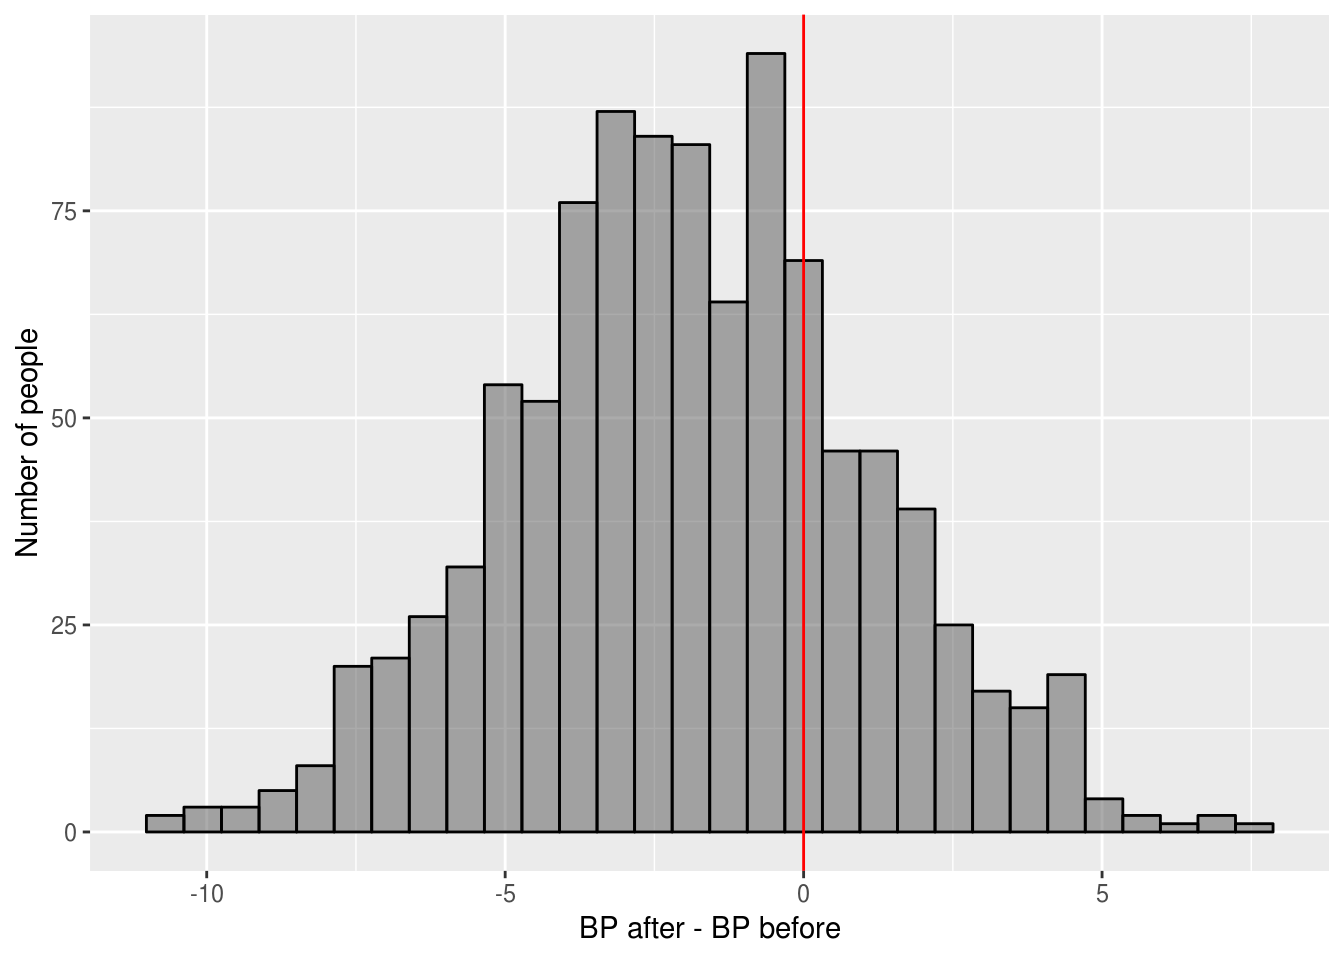
\includegraphics{website_files/figure-latex/unnamed-chunk-5-1.pdf}

\newpage

\subsubsection{Example 2}\label{example-2-1}

\(\rightarrow\) Testing if there is a difference in mouse DNA damage
before and after irradiating (measured on the same mouse)

\[\text{H}_0: \mu_{\text{DNA damage after}-\text{DNA damage before}} = 0\]
\[\text{H}_1: \mu_{\text{DNA damage after}-\text{DNA damage before}} \ne 0\]

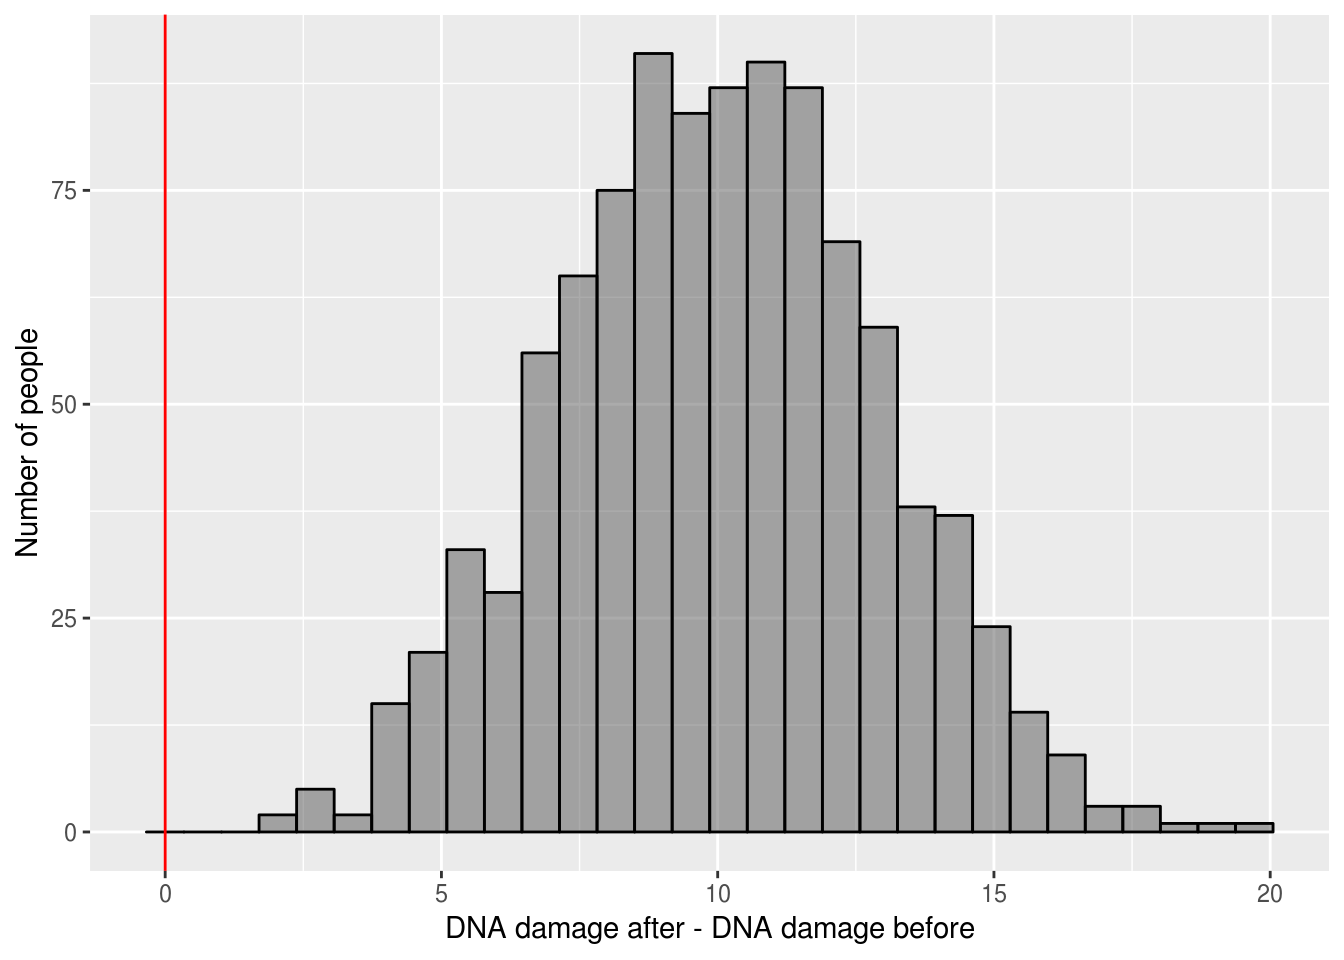
\includegraphics{website_files/figure-latex/unnamed-chunk-6-1.pdf}

\subsubsection{Example 3}\label{example-3-1}

\(\rightarrow\) \hfill \break
\hfill \break
\hfill \break
\(H_0:\) \hfill \break
\hfill \break
\hfill \break
\(H_1:\)

\newpage

\subsubsection{Example 4}\label{example-4-1}

\(\rightarrow\) \hfill \break
\hfill \break
\hfill \break
\(H_0:\) \hfill \break
\hfill \break
\hfill \break
\(H_1:\)

\subsubsection{Non-Parametric
Equivalent}\label{non-parametric-equivalent}

Wilcoxon signed-rank test. This should be used when the Normality
assumption fails.

\newpage

\subsection{Two-sample Unpaired
T-Test}\label{two-sample-unpaired-t-test}

An unpaired t-test is where we have two independent groups of \(N_1\)
and \(N_2\) participants, and we want to test if the mean of the outcome
variable differs between \(\text{group}_1\) and \(\text{group}_2\).

\[\text{H}_0: \mu_0 = \mu_1\] \[\text{H}_1: \mu_0 \ne \mu_1\]

Or rephrased:

\[\text{H}_0: \text{The average height of men is equal to the average height of women}\]
\[\text{H}_1: \text{The average height of men is not equal to the average height of women}\]

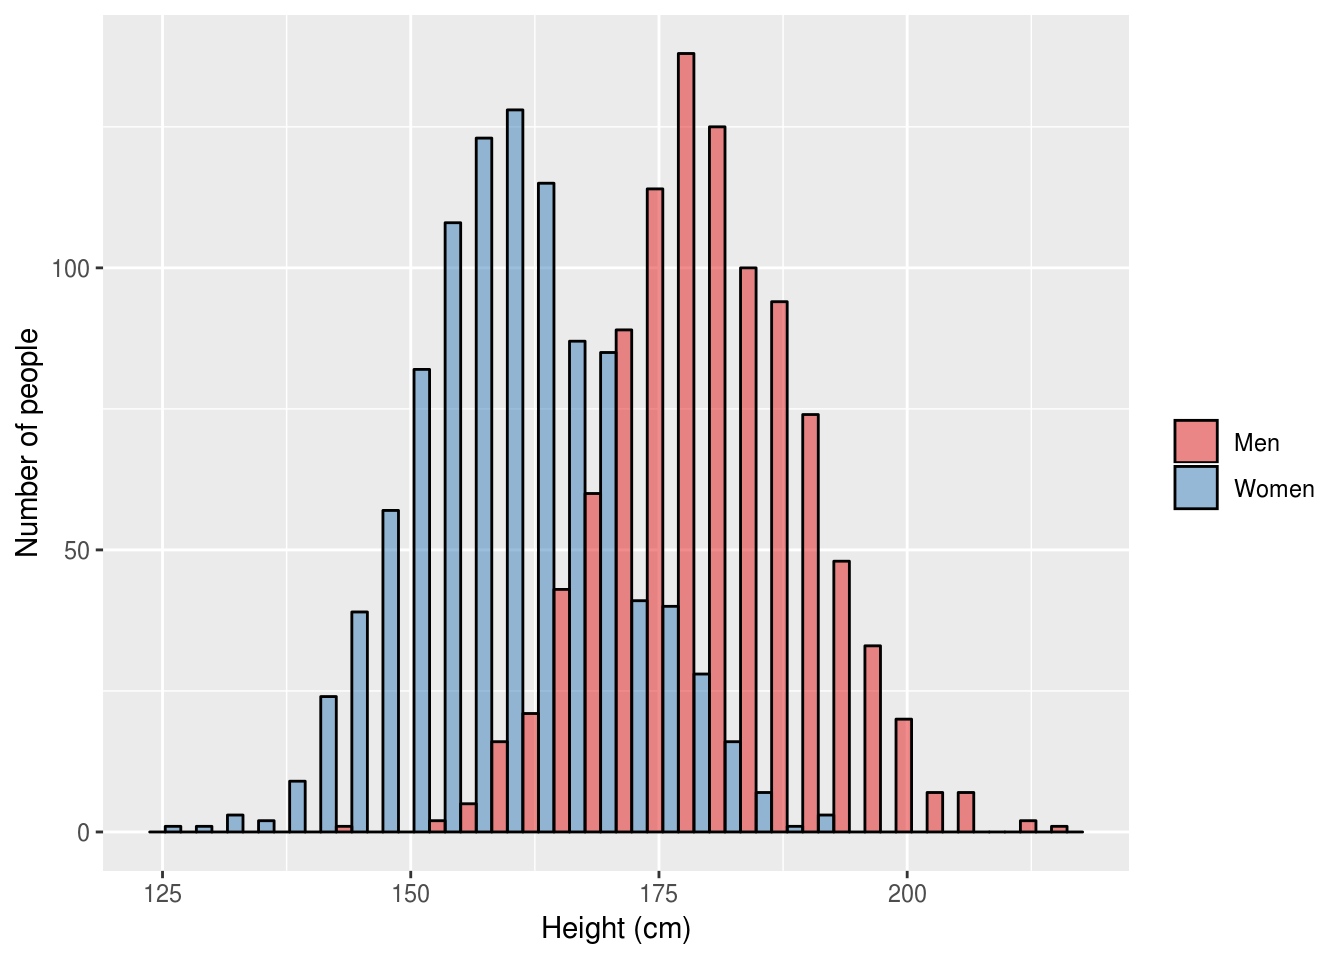
\includegraphics{website_files/figure-latex/unnamed-chunk-7-1.pdf}

\subsubsection{Aim/Outcome/Exposure/Parametric/Dependencies}\label{aimoutcomeexposureparametricdependencies-3}

\textbf{Aim}: Hypothesis testing (test if the mean of a continuous
variable differs between \(\text{group}_1\) and \(\text{group}_2\))

\textbf{Outcome}: continuous variable

\textbf{Exposure}: \(\text{group}_1\) vs \(\text{group}_2\)

\textbf{Parametric assumptions}: Outcomes for each group are distributed
as a Normal distribution

\textbf{Dependencies}: None (all observations independent)

\newpage

\subsubsection{Example 1}\label{example-1-2}

\(\rightarrow\) Testing if the average blood pressure in people who
didn't receive treatment is different from people who did receive
treatment

\[\text{H}_0: \mu_{\text{BP treatment}} = \mu_{\text{BP no treatment}}\]
\[\text{H}_1: \mu_{\text{BP treatment}} \ne \mu_{\text{BP no treatment}}\]

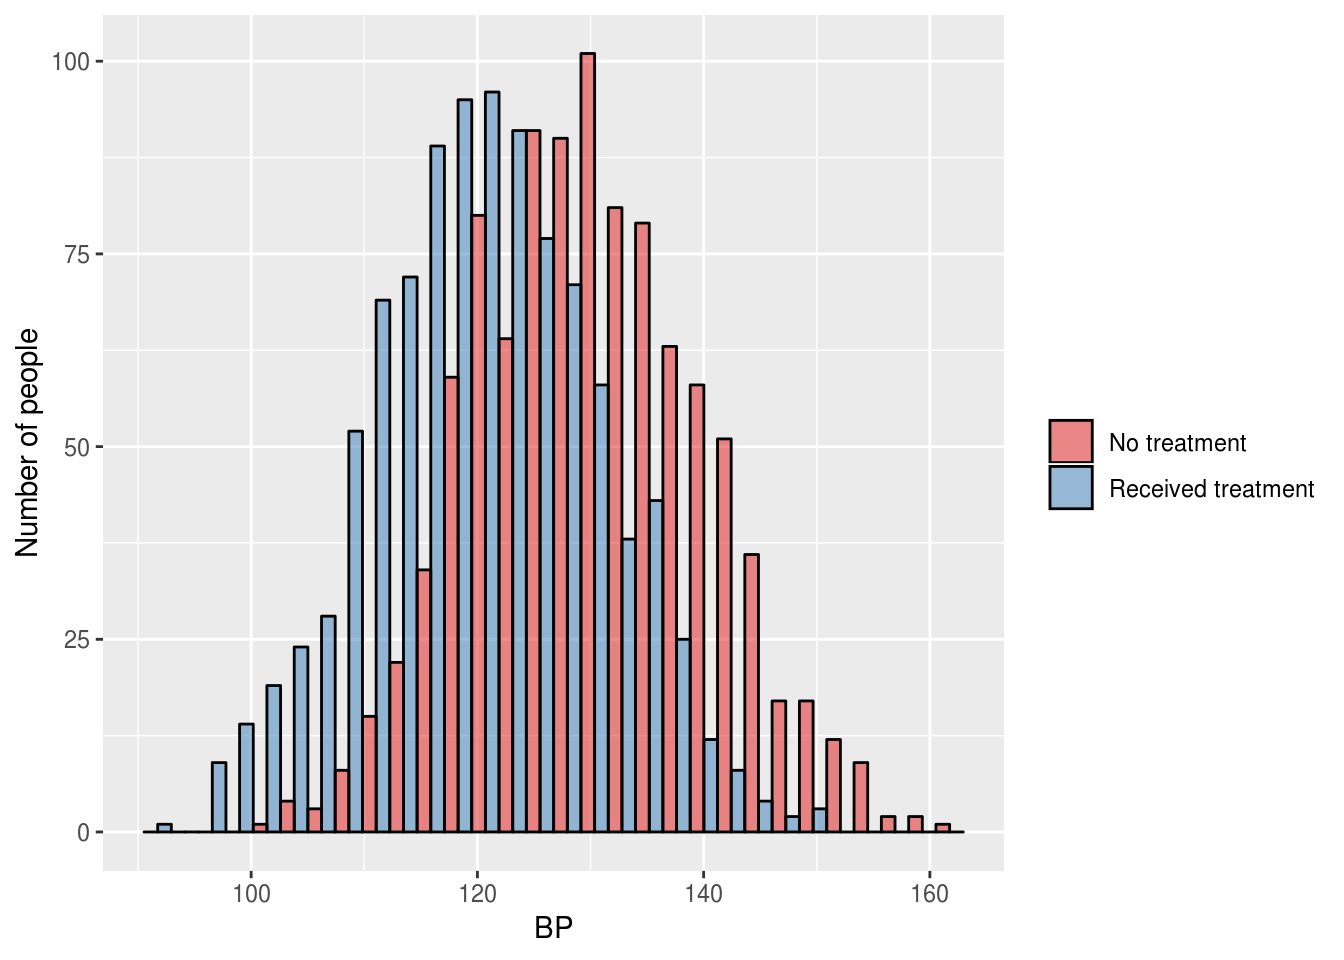
\includegraphics{website_files/figure-latex/unnamed-chunk-8-1.pdf}

\newpage

\subsubsection{Example 2}\label{example-2-2}

\(\rightarrow\) Testing if the average DNA damage in mice that weren't
irradiated is different from mice that were irradiated

\[\text{H}_0: \mu_{\text{DNA radiation}} = \mu_{\text{DNA no radiation}}\]
\[\text{H}_1: \mu_{\text{DNA radiation}} \ne \mu_{\text{DNA no radiation}}\]

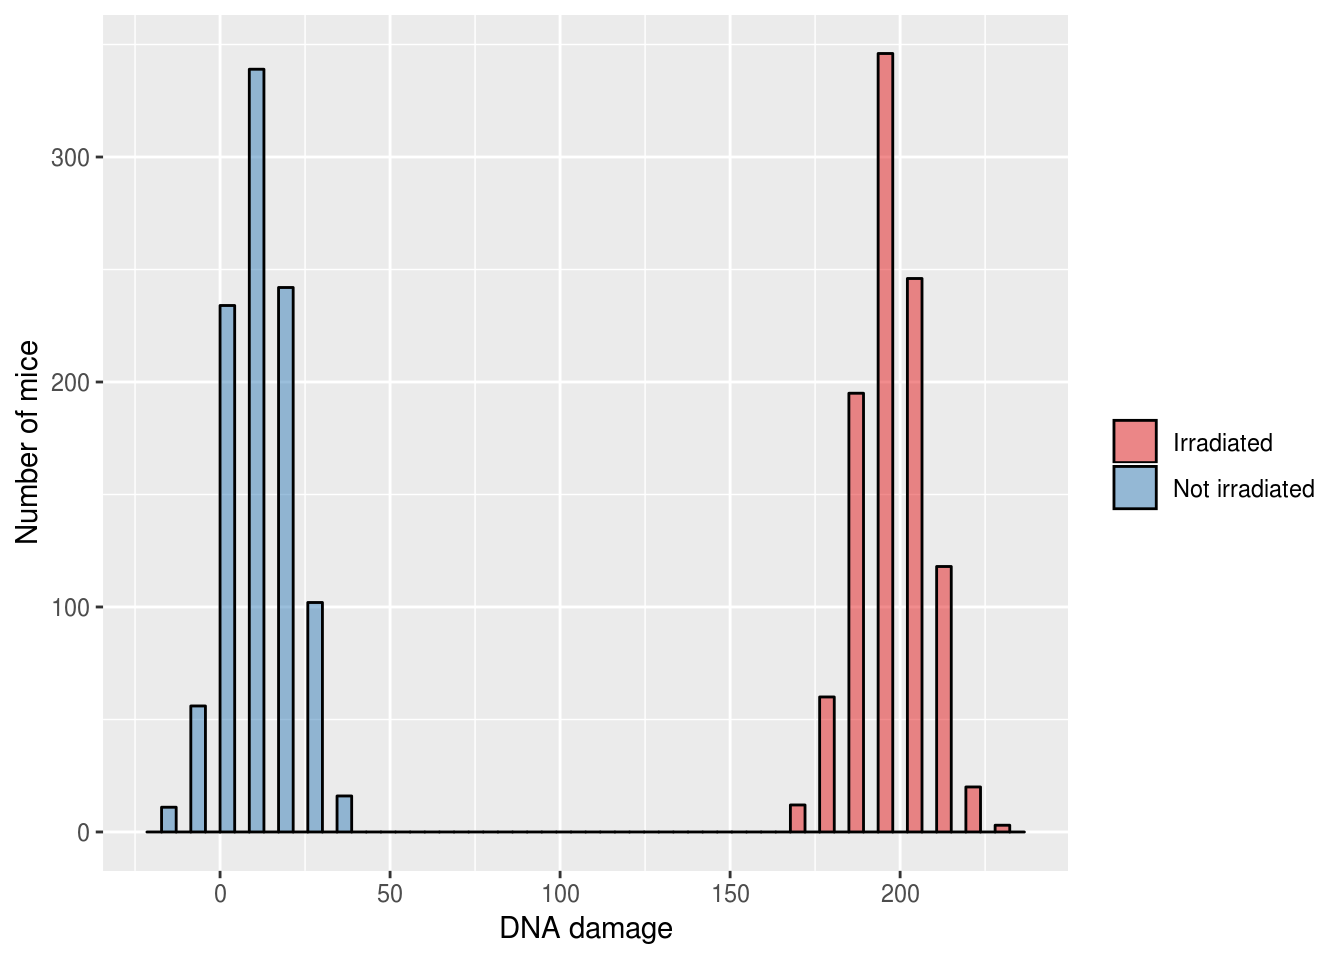
\includegraphics{website_files/figure-latex/unnamed-chunk-9-1.pdf}

\subsubsection{Example 3}\label{example-3-2}

\(\rightarrow\) \hfill \break
\hfill \break
\hfill \break
\(H_0:\) \hfill \break
\hfill \break
\hfill \break
\(H_1:\)

\newpage

\subsubsection{Example 4}\label{example-4-2}

\(\rightarrow\) \hfill \break
\hfill \break
\hfill \break
\(H_0:\) \hfill \break
\hfill \break
\hfill \break
\(H_1:\)

\subsubsection{Non-parametric
equivalent}\label{non-parametric-equivalent-1}

Mann--Whitney U test (also called the Mann--Whitney--Wilcoxon (MWW),
Wilcoxon rank-sum test, or Wilcoxon--Mann--Whitney test). This should be
used when the Normality assumption fails.

\subsection{ANOVA}\label{anova}

ANOVA is an extension of the two-sample unpaired t-test. We have X
independent groups of participants, and we want to test if the mean of
the outcome variable differs between groups.

\subsubsection{Aim/Outcome/Exposure/Parametric/Dependencies}\label{aimoutcomeexposureparametricdependencies-4}

\textbf{Aim}: Hypothesis testing (test if the mean of a continuous
variable differs between some groups)

\textbf{Outcome}: continuous variable

\textbf{Exposure}: \(\text{group}_1\) vs \(\text{group}_2\) (vs
\(\text{group}_3\) \ldots{})

\textbf{Parametric assumptions}: Outcomes for each group are distributed
as a Normal distribution

\textbf{Dependencies}: None (all observations independent)

\newpage

\subsubsection{Example 1}\label{example-1-3}

\(\rightarrow\) Testing if average BMI levels differ across Scandinavia

\[\text{H}_0: \mu_{\text{Norway}} = \mu_{\text{Denmark}} = \mu_{\text{Sweden}}\]
\[\text{H}_1: \mu_{\text{Norway}} \ne \mu_{\text{Denmark}} \text{ and/or } \mu_{\text{Norway}} \ne \mu_{\text{Sweden}}  \text{ and/or } \mu_{\text{Denmark}} \ne \mu_{\text{Sweden}}\]

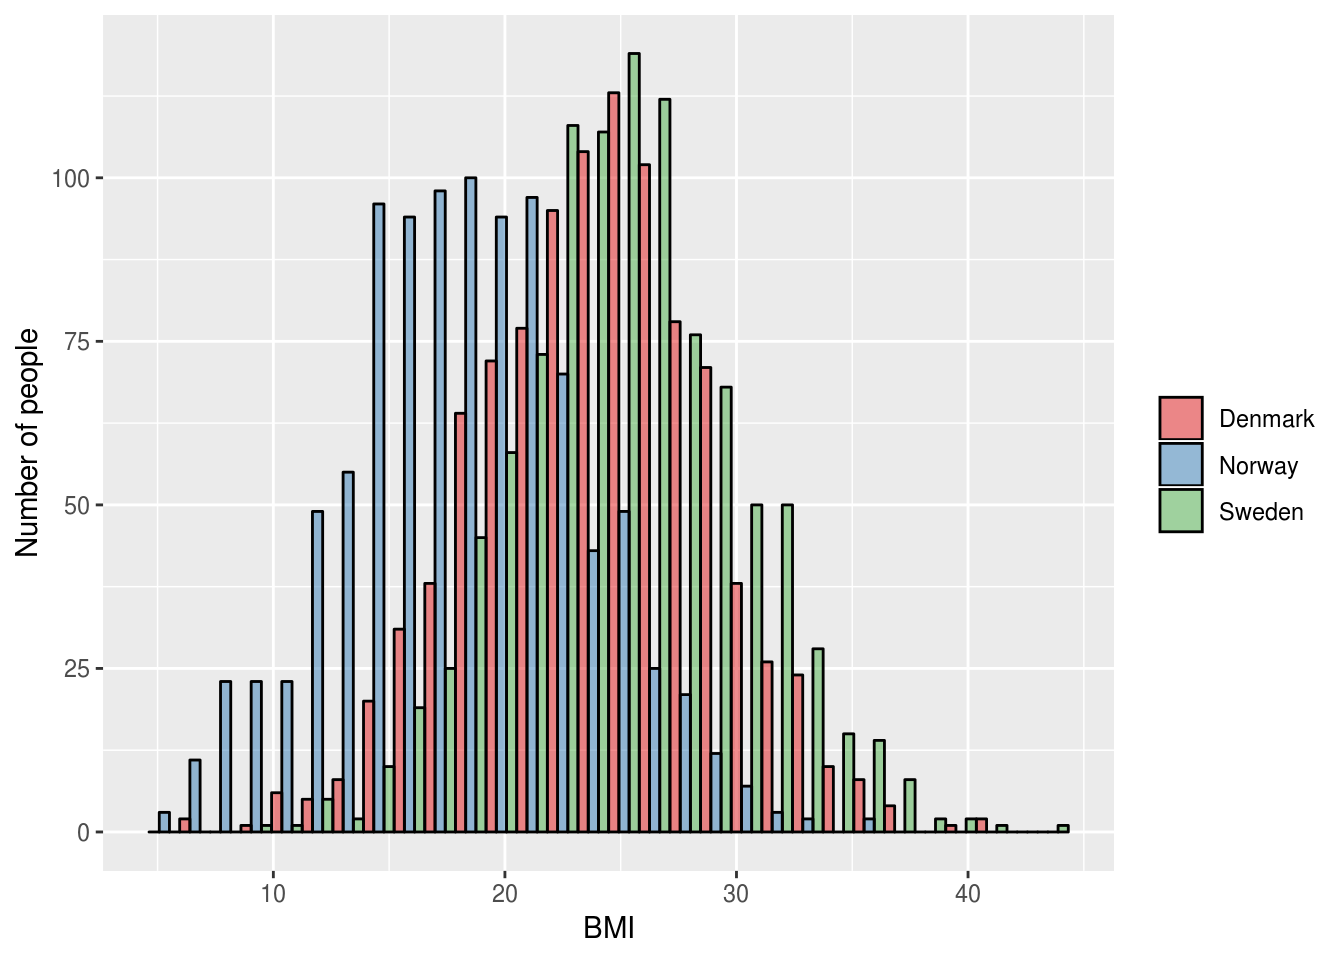
\includegraphics{website_files/figure-latex/unnamed-chunk-10-1.pdf}

\newpage

\subsubsection{Example 2}\label{example-2-3}

\(\rightarrow\) Testing if average water pH levels differ between East
and West Oslo

\[\text{H}_0: \mu_{\text{East Oslo}} = \mu_{\text{West Oslo}}\]
\[\text{H}_1: \mu_{\text{East Oslo}} \ne \mu_{\text{West Oslo}}\]

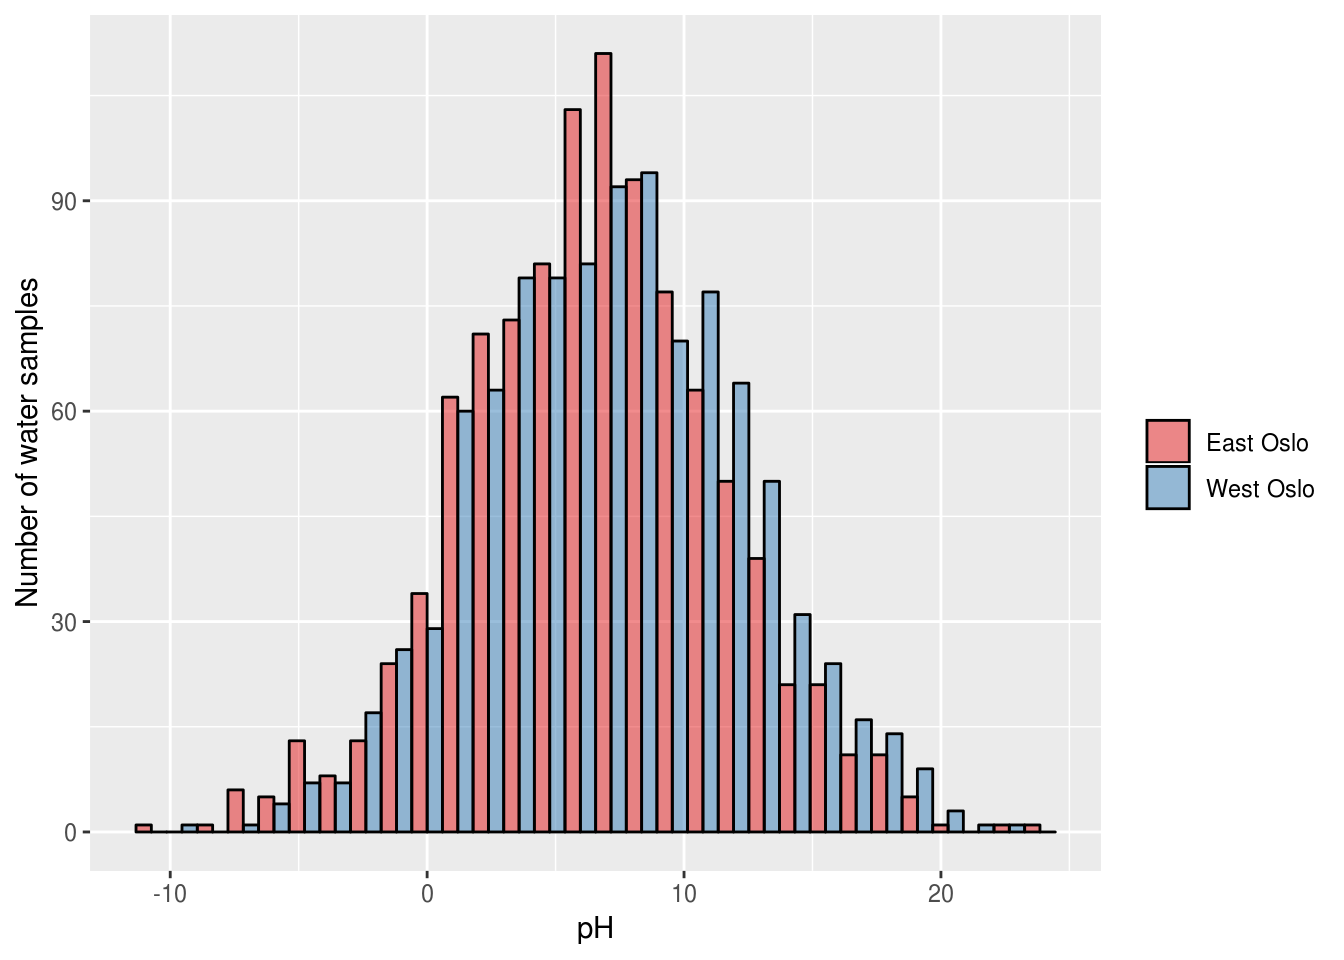
\includegraphics{website_files/figure-latex/unnamed-chunk-11-1.pdf}

\subsubsection{Example 3}\label{example-3-3}

\(\rightarrow\) \hfill \break
\hfill \break
\hfill \break
\(H_0:\) \hfill \break
\hfill \break
\hfill \break
\(H_1:\)

\newpage

\subsubsection{Example 4}\label{example-4-3}

\(\rightarrow\) \hfill \break
\hfill \break
\hfill \break
\(H_0:\) \hfill \break
\hfill \break
\hfill \break
\(H_1:\)

\subsubsection{Non-parametric
equivalent}\label{non-parametric-equivalent-2}

Kruskal--Wallis test

\section{Simple regression (fixed
effects)}\label{simple-regression-fixed-effects}

\subsection{Regression in general}\label{regression-in-general}

Regression is the explicit modelling of a parametric association between
an outcome and an exposure.

One such parametric association might be the following:

\[\text{outcome} = 3 + 2 \times \text{exposure}\]

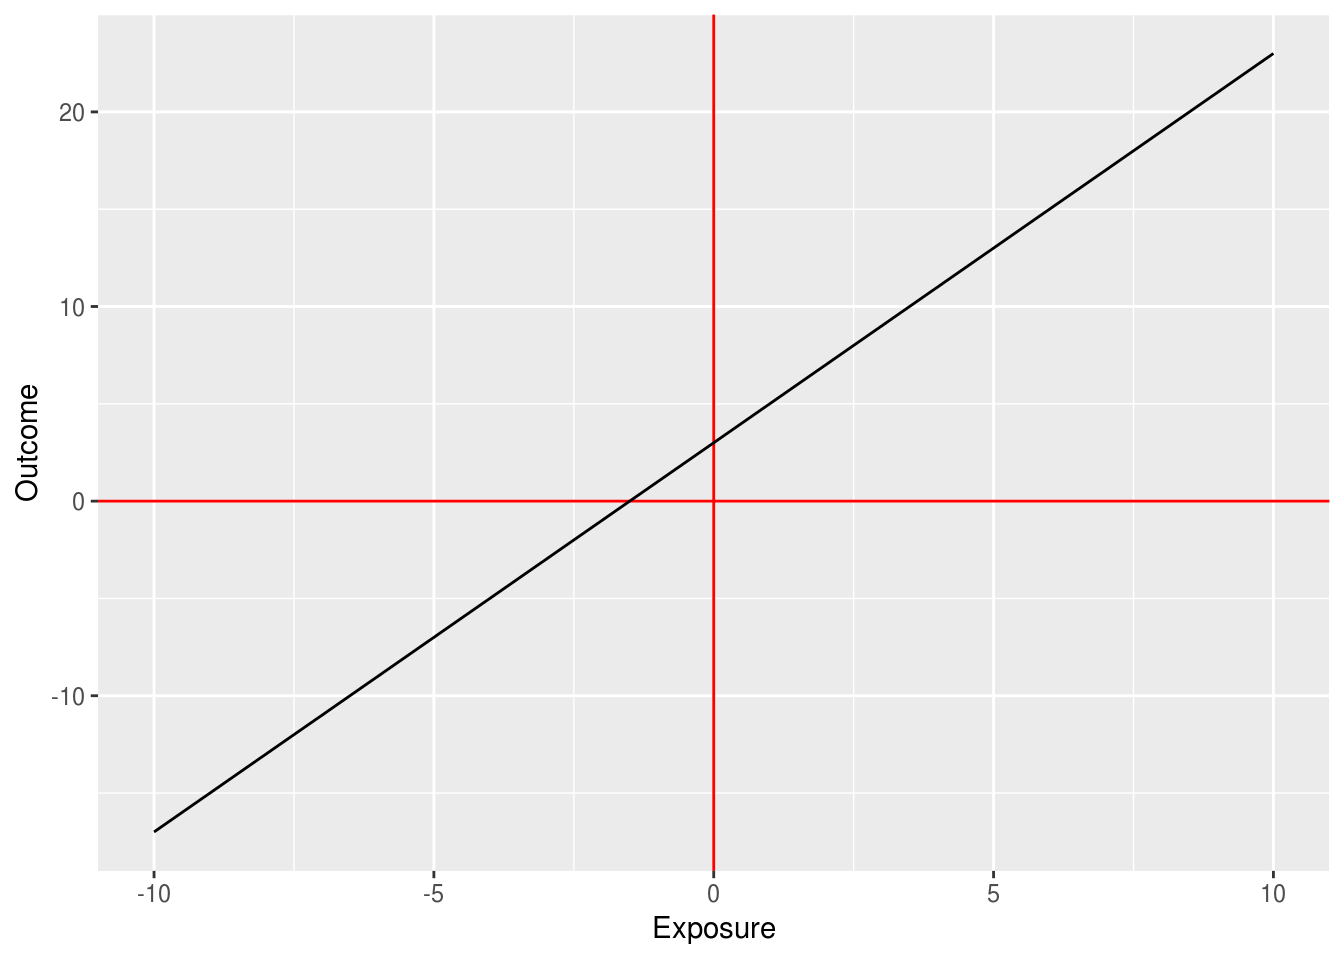
\includegraphics{website_files/figure-latex/unnamed-chunk-12-1.pdf}

Depending on the type of outcome, different types of regression will
need to be used.

For all regressions, the exposure can be:

\begin{itemize}
\tightlist
\item
  Continuous
\item
  Binary (0 or 1)
\item
  Categorical (0, 1, 2, \ldots{})
\item
  Count data
\end{itemize}

Regressions can both:

\begin{itemize}
\tightlist
\item
  Perform hypothesis testing (same as the previous tests we have learned
  about)
\item
  Estimate numerically the effect size of the association between
  outcome and exposure (new!)
\end{itemize}

\subsection{Linear regression}\label{linear-regression}

In the most basic form, we have:

\[\text{outcome} = \beta_0 + \beta_1 \times \text{exposure} + \text{error}\]

Where we aim to estimate values for \(\beta_0\) and \(\beta_1\).

For example, if we run an ice cream shop:

\[\text{number of ice creams sold} = 5 + 3 \times \text{temperature} + \text{error}\]

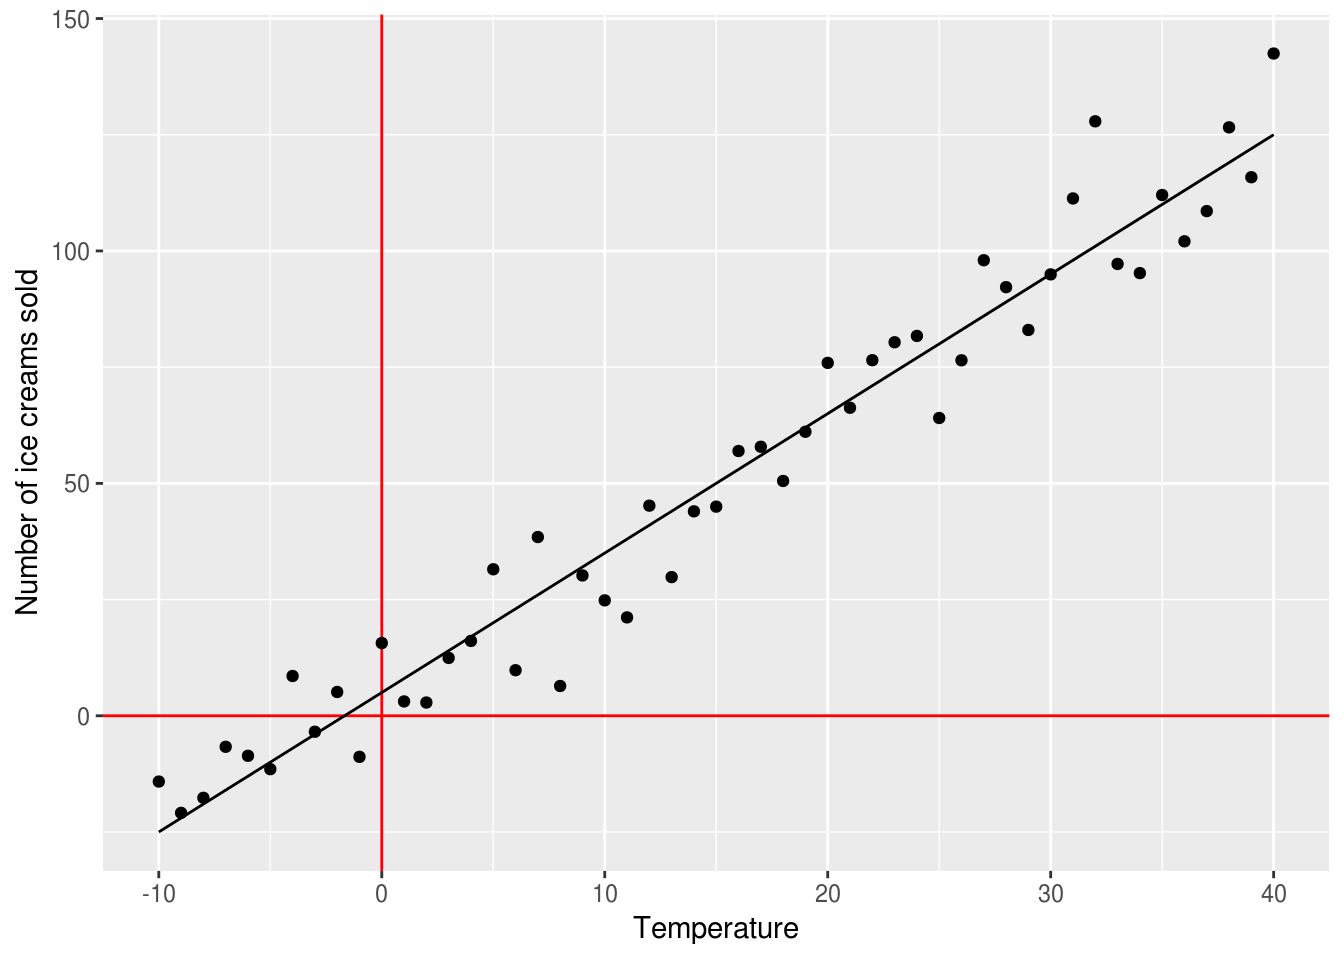
\includegraphics{website_files/figure-latex/unnamed-chunk-13-1.pdf}

If today's temperature is 30C, we can expect our shop to sell
\(5 + 3 \times 30 = 95\) ice creams. Because \(\beta_1\) (\(=3\)) was
not zero, we have a significant association between temperature and
number of ice creams sold.

Another example, if we work as a midwife:

\[\text{Child's birthweight} = 3 + 0 \times \text{temperature at day of delivery} + \text{error}\]

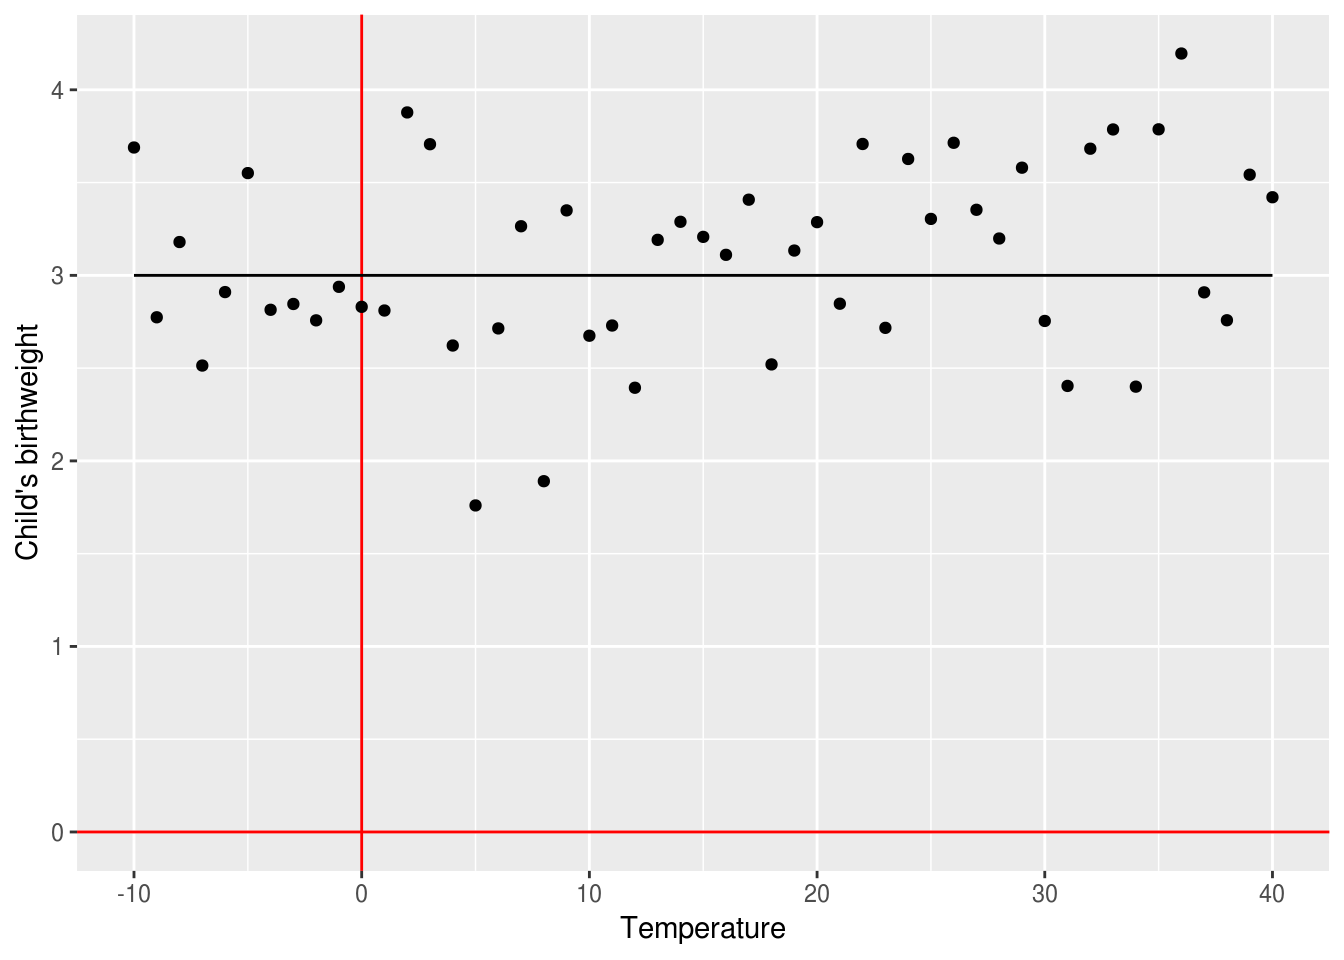
\includegraphics{website_files/figure-latex/unnamed-chunk-14-1.pdf}

If today's temperature is 30C, we can expect that children born today
will be (on average) \(3 + 0 \times 30 = 3\) kg. If tomorrow's
temperature is 10C, we can expect that children born today will be (on
average) \(3 + 0 \times 10 = 3\) kg. Because \(\beta_1\) was zero, we do
not have a significant association between temperature and birthweight.

\subsubsection{Aim/Outcome/Exposure/Parametric/Dependencies}\label{aimoutcomeexposureparametricdependencies-5}

\textbf{Aim}: Hypothesis testing and estimating the effect size of the
association between outcome and exposure

\textbf{Outcome}: \emph{Continuous variable}

\textbf{Exposure}: Continuous, Binary, Categorical, Count variable

\textbf{Parametric assumptions}: Residuals are distributed as a Normal
distribution

\textbf{Dependencies}: None (all observations independent)

\newpage

\subsubsection{Example 1}\label{example-1-4}

\(\rightarrow\) Testing if average birth weight (continuous outcome) is
associated with parents' income (continuous exposure)

\[\text{birth weight} = \beta_0 + \beta_1 \times \text{parent's income} + \text{error}\]

\[\text{H}_0: \beta_1 = 0\] \[\text{H}_1: \beta_1 \ne 0\]

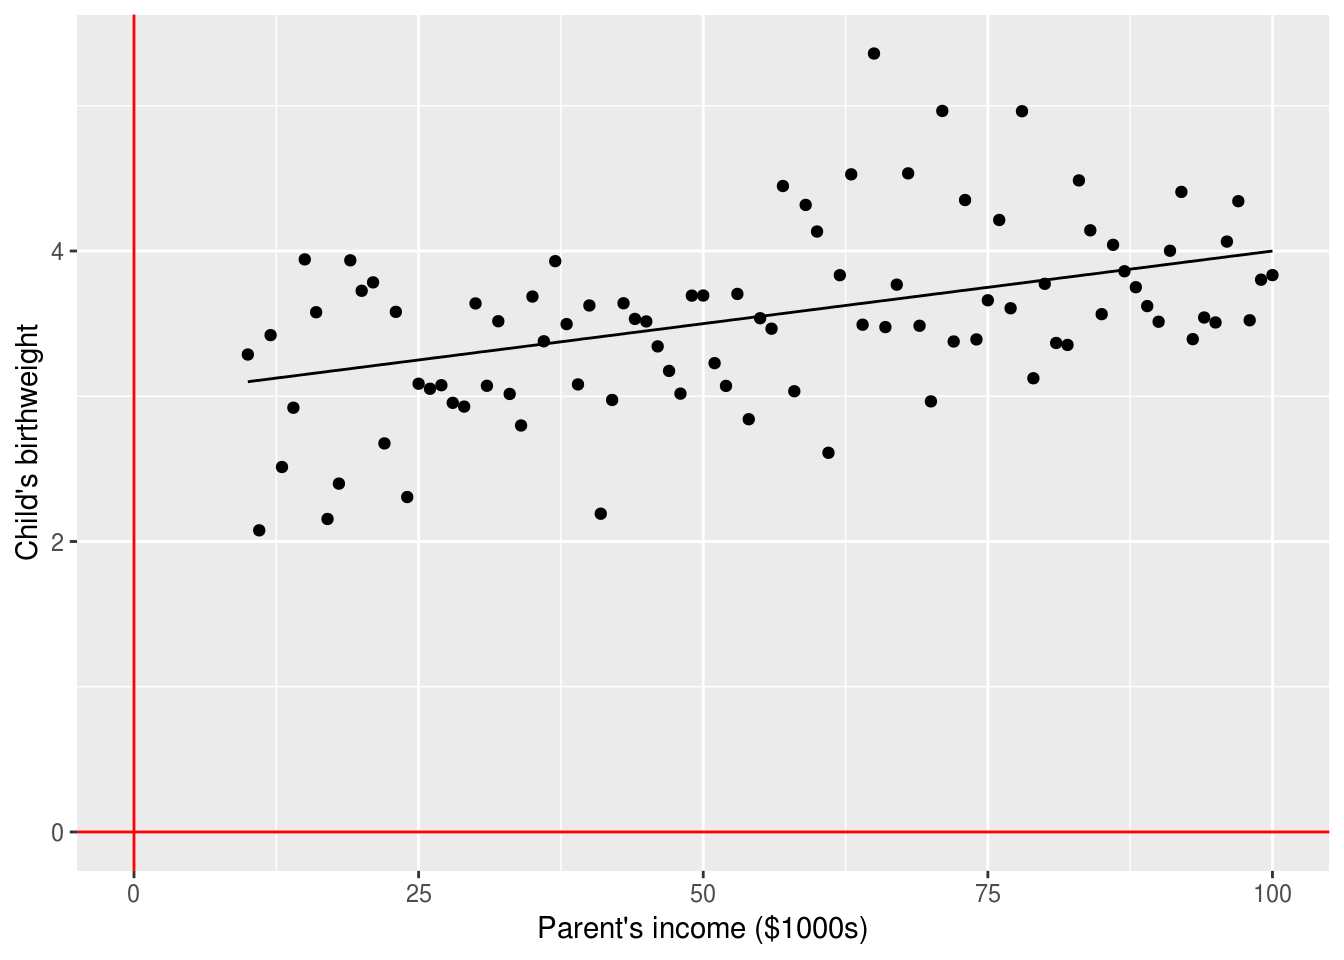
\includegraphics{website_files/figure-latex/unnamed-chunk-15-1.pdf}

\newpage

\subsubsection{Example 2}\label{example-2-4}

\(\rightarrow\) Testing if average birth weight (continuous outcome) is
associated with child's sex (binary exposure)

\[\text{birth weight} = \beta_0 + \beta_1 \times \text{is boy} + \text{error}\]

\[\text{H}_0: \beta_1 = 0\] \[\text{H}_1: \beta_1 \ne 0\]

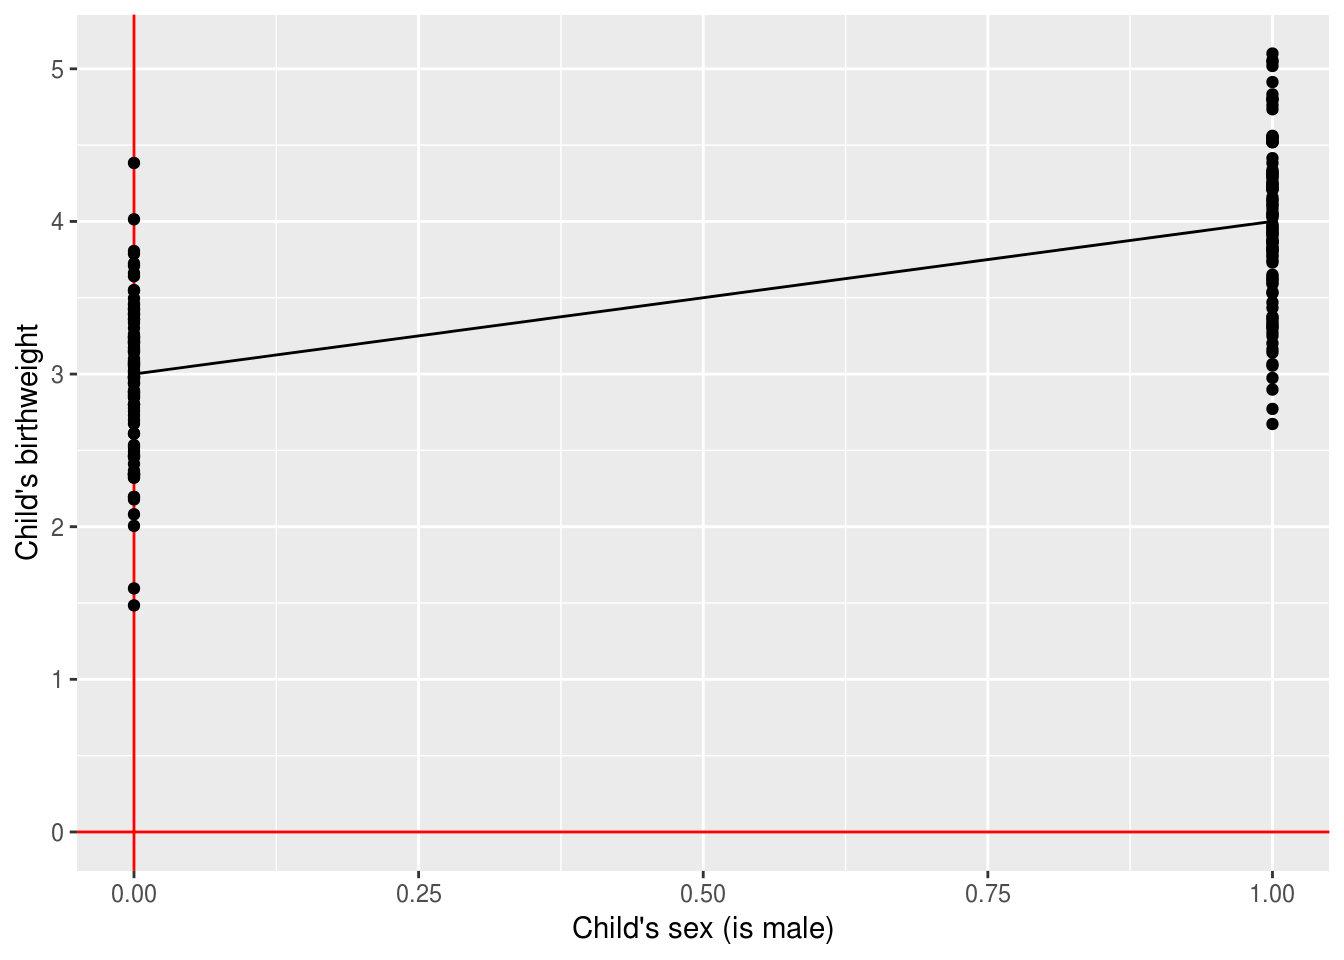
\includegraphics{website_files/figure-latex/unnamed-chunk-16-1.pdf}

\newpage

\subsubsection{Example 3}\label{example-3-4}

\(\rightarrow\) Testing if average BMI levels (continuous outcome)
differ across Scandinavia (categorical exposure)

\[\text{bmi} = \beta_0 + \beta_1 \times \text{is Norway} + \beta_2 \times \text{is Sweden} + \text{error}\]

\[\text{H}_0: \beta_1 = \beta_2 = 0\]
\[\text{H}_1: \beta_1 \ne 0 \text{ and/or } \beta_2 \ne 0\]

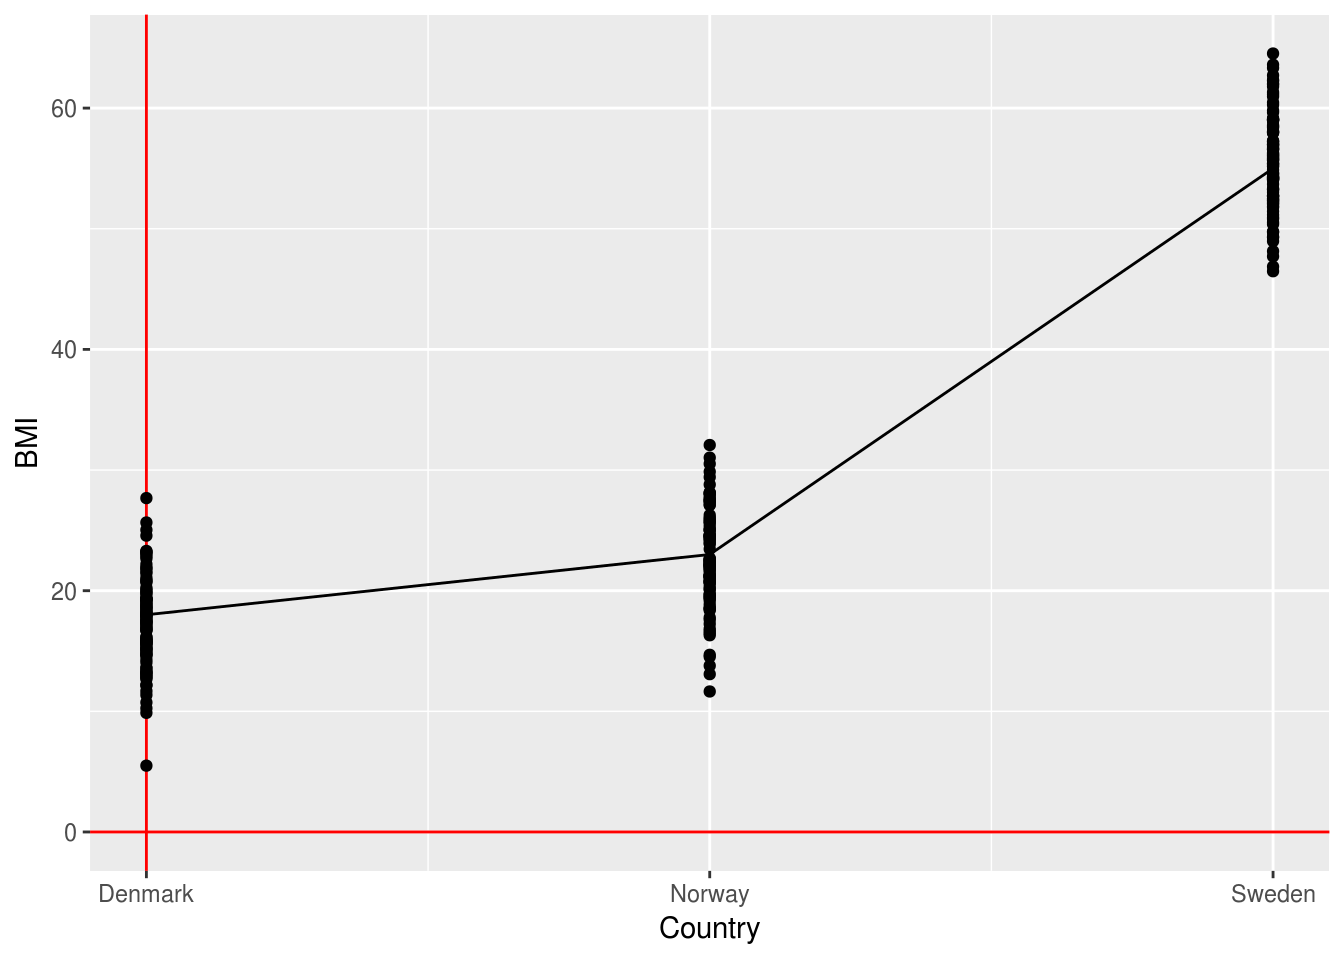
\includegraphics{website_files/figure-latex/unnamed-chunk-17-1.pdf}

\subsubsection{Example 4}\label{example-4-4}

\(\rightarrow\) \hfill \break
\hfill \break
\hfill \break
\hfill \break
\hfill \break
\hfill \break
\(H_0:\) \hfill \break
\hfill \break
\hfill \break
\(H_1:\)

\subsubsection{Example 5}\label{example-5}

\(\rightarrow\) \hfill \break
\hfill \break
\hfill \break
\hfill \break
\hfill \break
\hfill \break
\(H_0:\) \hfill \break
\hfill \break
\hfill \break
\(H_1:\)

\newpage

\subsection{Similarities between t-tests, ANOVA, and linear
regression}\label{similarities-between-t-tests-anova-and-linear-regression}

\subsubsection{Example 1}\label{example-1-5}

\textbf{Two-sample unpaired t-test}:

\(\rightarrow\) Testing if average birth weight (continuous outcome) is
different in female children versus male children

\[\text{H}_0: \mu_{\text{boys}} = \mu_{\text{girls}}\]
\[\text{H}_1: \mu_{\text{boys}} \ne \mu_{\text{girls}}\]

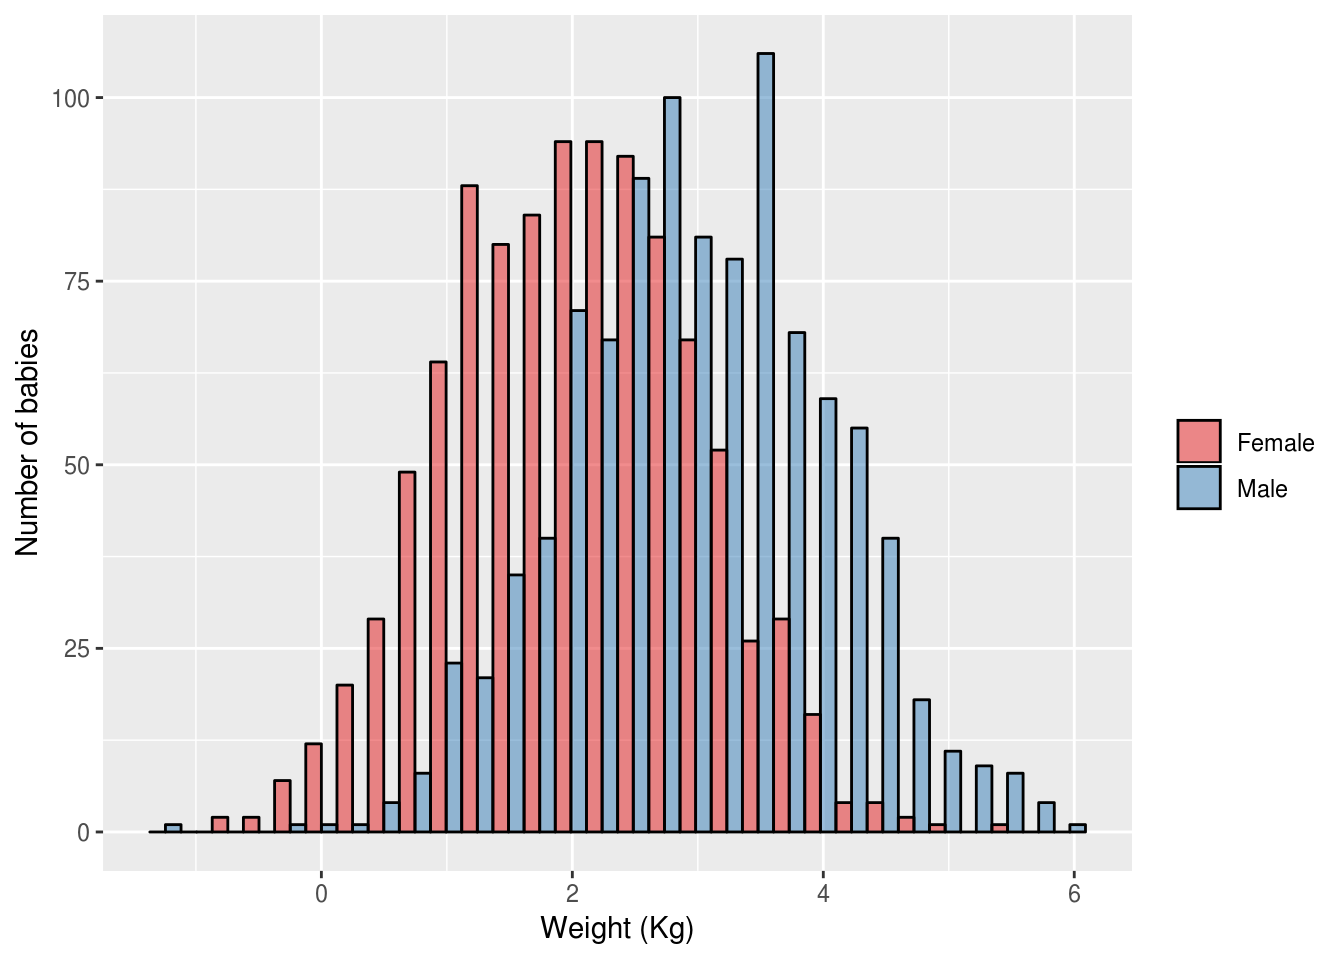
\includegraphics{website_files/figure-latex/unnamed-chunk-18-1.pdf}

\newpage

\textbf{ANOVA}:

\(\rightarrow\) Testing if average birth weight (continuous outcome) is
different in female children versus male children

\[\text{H}_0: \mu_{\text{boys}} = \mu_{\text{girls}}\]
\[\text{H}_1: \mu_{\text{boys}} \ne \mu_{\text{girls}}\]

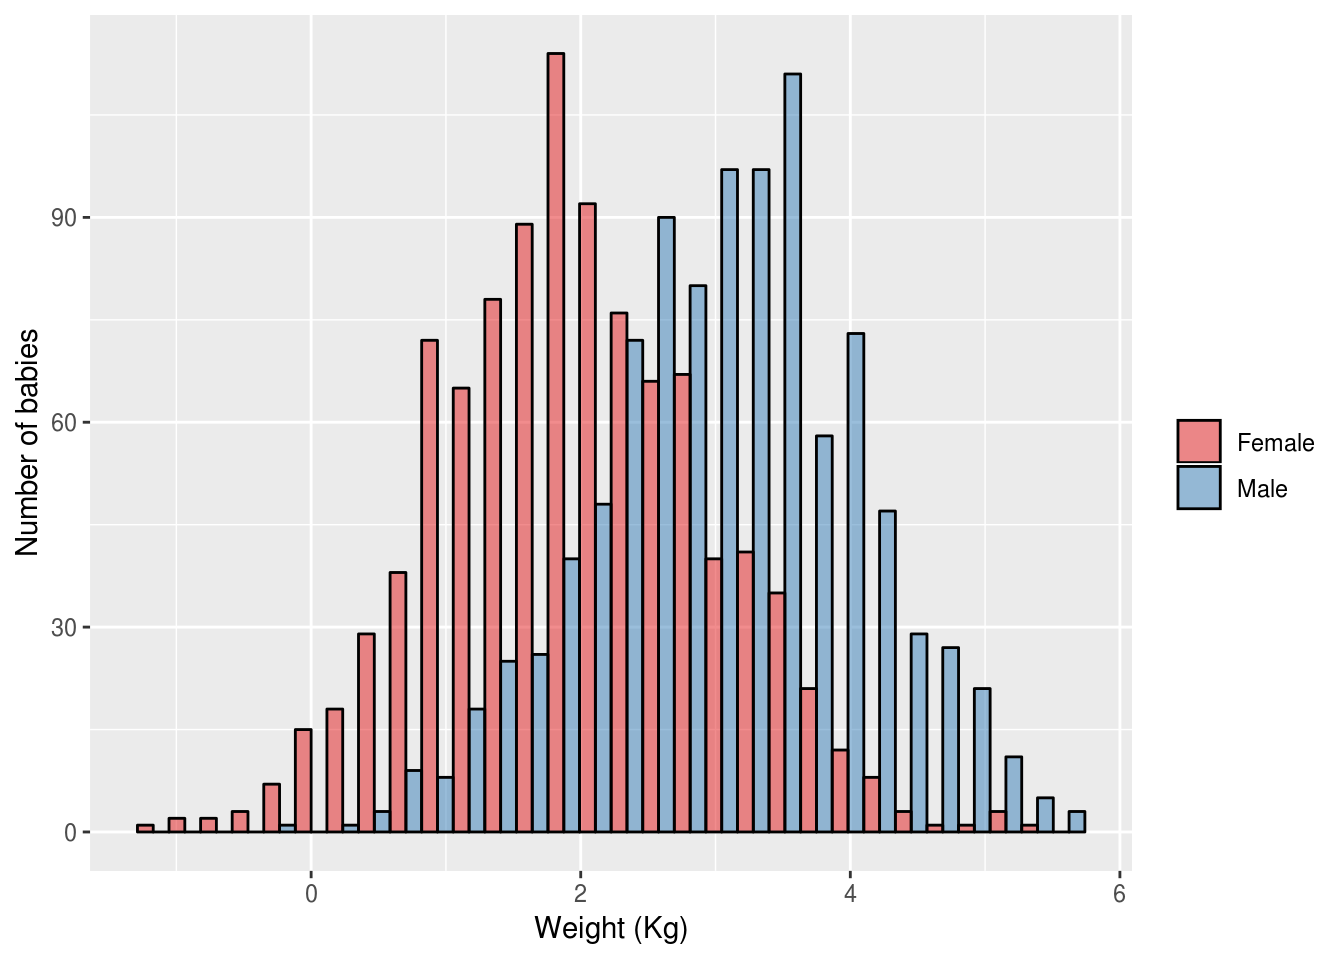
\includegraphics{website_files/figure-latex/unnamed-chunk-19-1.pdf}

\newpage

\textbf{Linear regression}:

\(\rightarrow\) Testing if the effect of child's sex on average birth
weight (continuous outcome) is different than zero

\[\text{birth weight} = \beta_0 + \beta_1 \times \text{is boy} + \text{error}\]
\[\text{H}_0: \beta_1 = 0\] \[\text{H}_1: \beta_1 \ne 0\]

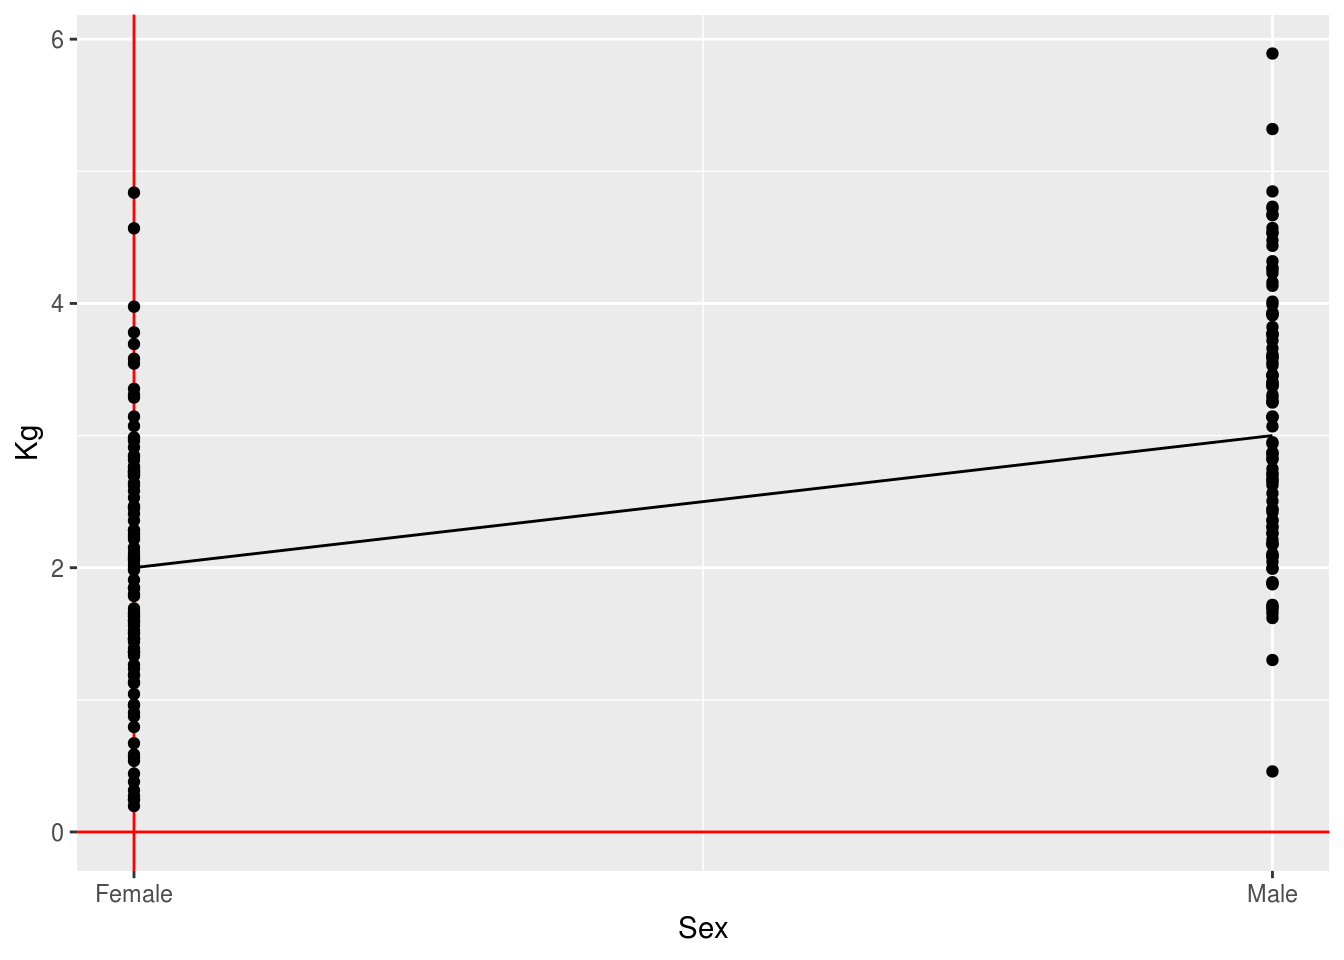
\includegraphics{website_files/figure-latex/unnamed-chunk-20-1.pdf}

\textbf{Conclusion}:

\begin{itemize}
\tightlist
\item
  Two-sample unpaired t-tests are ANOVAs with only two groups
\item
  Two-sample unpaired t-tests are linear regressions with a binary (0/1)
  exposure
\item
  ANOVA is a linear regression with a categorical exposure
\end{itemize}

\newpage

\subsubsection{Example 2}\label{example-2-5}

\textbf{Two-sample unpaired t-test}:

\(\rightarrow\) Testing if average number of hours sleep (continuous
outcome) is different in adults who are parents versus those who are
childless

\[\text{H}_0: \mu_{\text{parents}} = \mu_{\text{childless}}\]
\[\text{H}_1: \mu_{\text{parents}} \ne \mu_{\text{childless}}\]

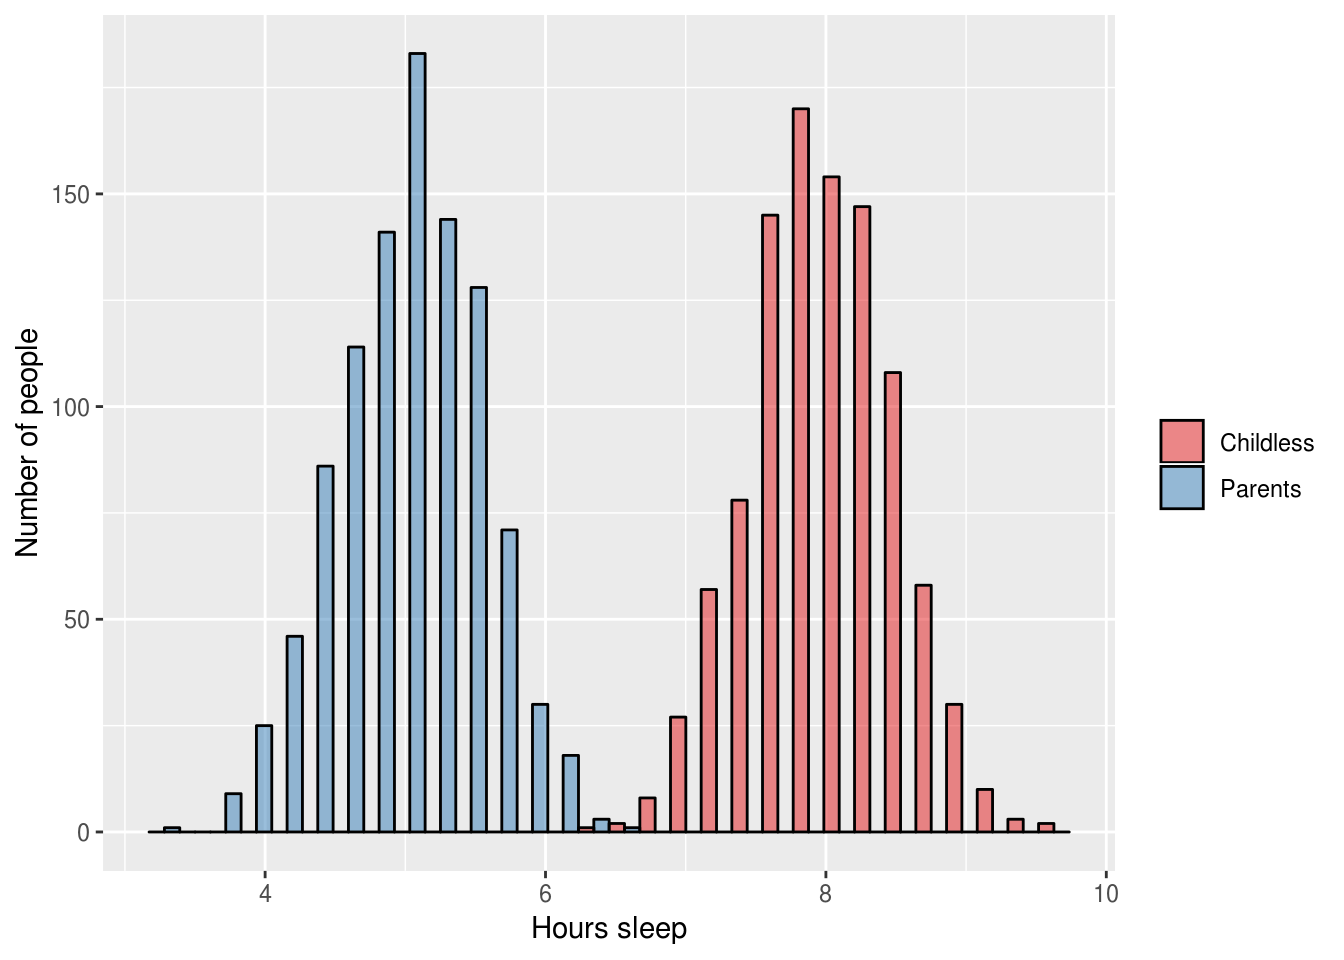
\includegraphics{website_files/figure-latex/unnamed-chunk-21-1.pdf}

\newpage

\textbf{ANOVA}:

\(\rightarrow\) Testing if average number of hours sleep (continuous
outcome) is different in adults who are parents versus those who are
childless

\[\text{H}_0: \mu_{\text{parents}} = \mu_{\text{childless}}\]
\[\text{H}_1: \mu_{\text{parents}} \ne \mu_{\text{childless}}\]

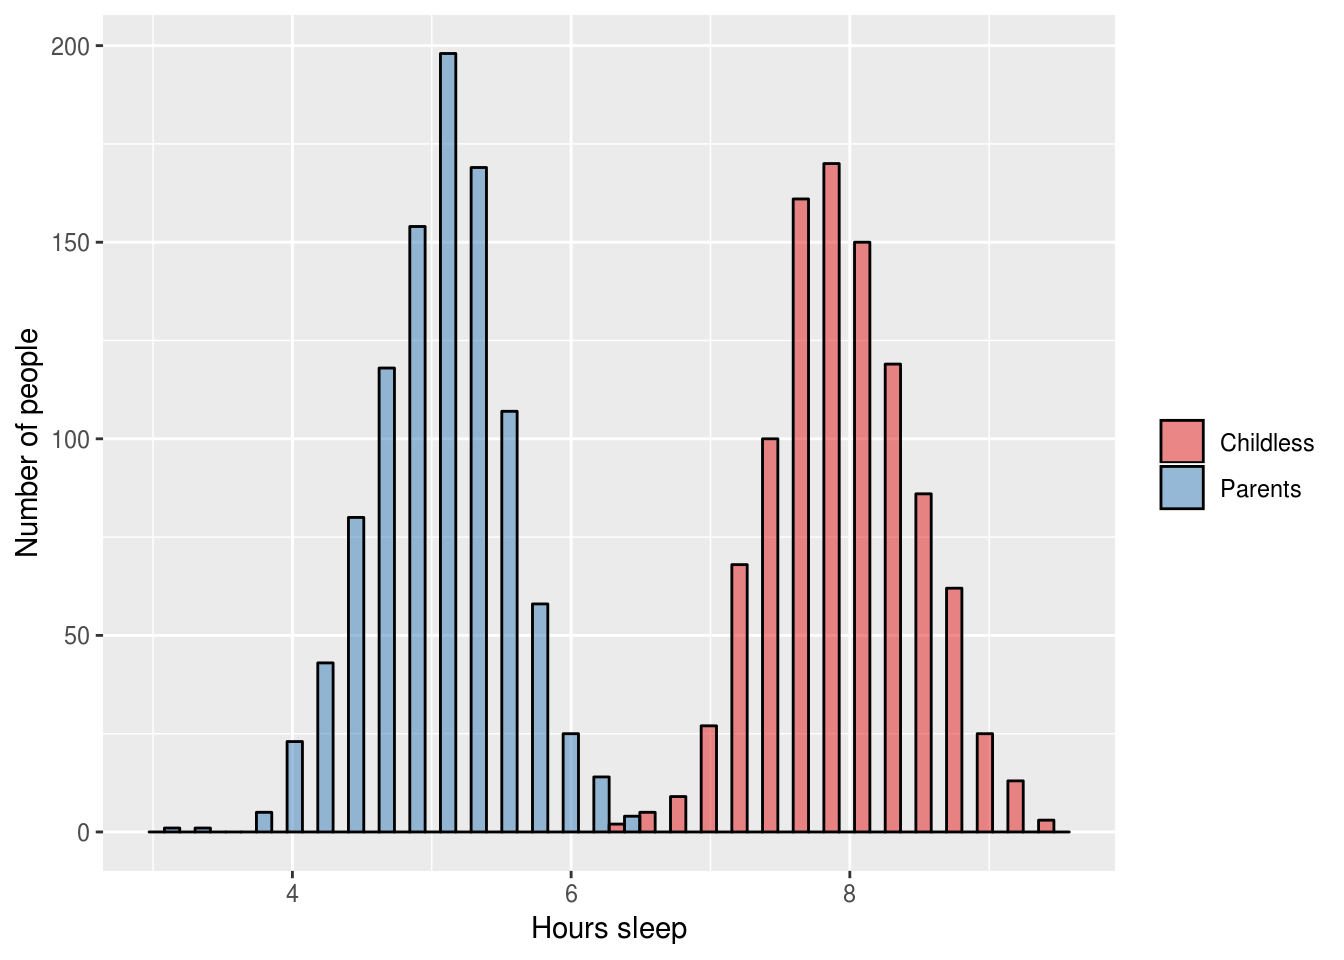
\includegraphics{website_files/figure-latex/unnamed-chunk-22-1.pdf}

\newpage

\textbf{Linear regression}:

\(\rightarrow\) Testing if the effect of being a parent on average
number of hours sleep (continuous outcome) is different than zero

\[\text{birth weight} = \beta_0 + \beta_1 \times \text{is parent} + \text{error}\]
\[\text{H}_0: \beta_1 = 0\] \[\text{H}_1: \beta_1 \ne 0\]

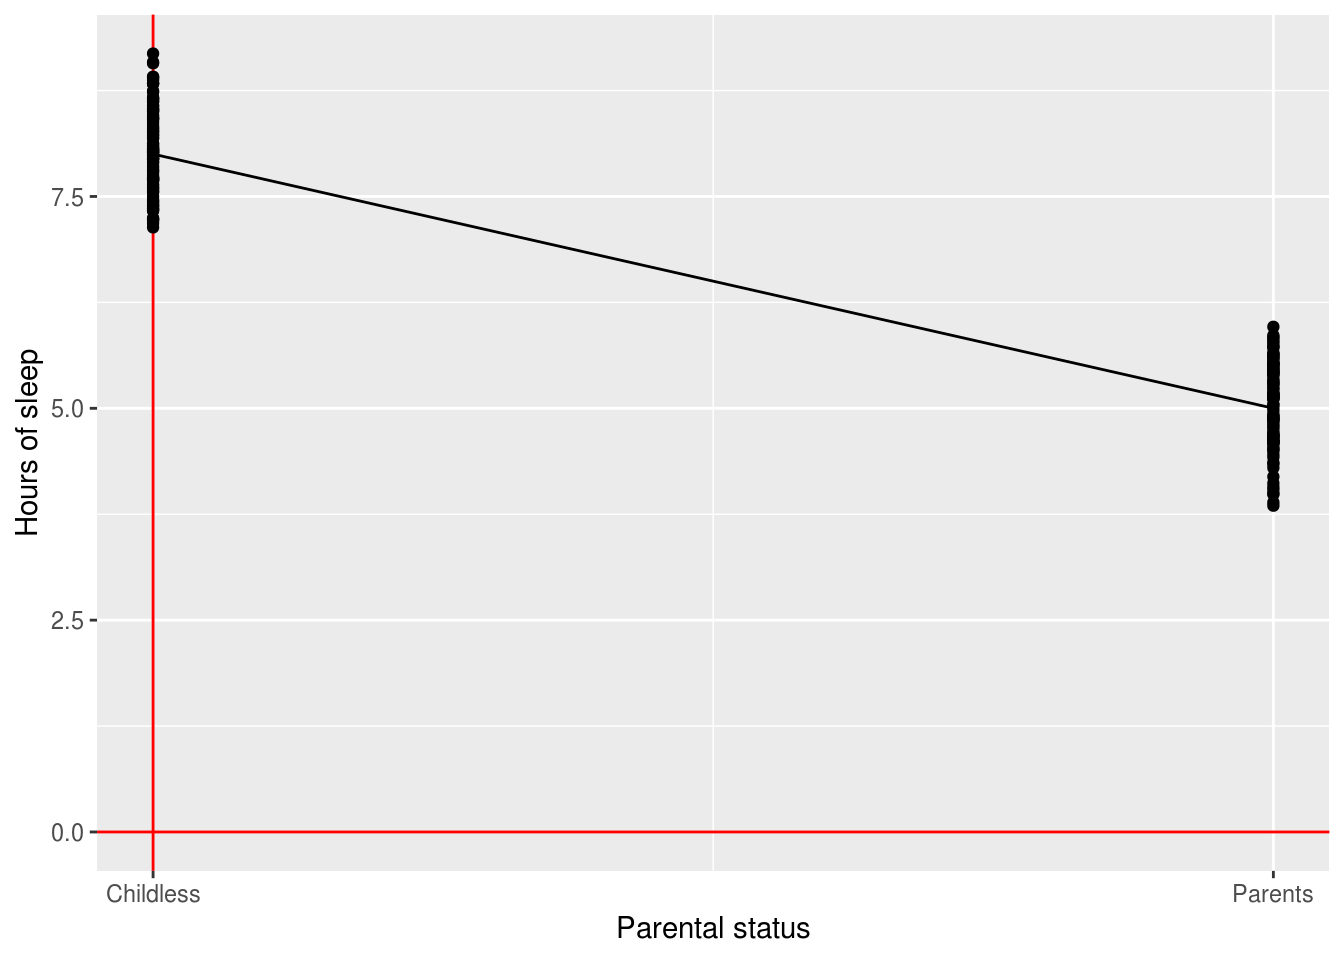
\includegraphics{website_files/figure-latex/unnamed-chunk-23-1.pdf}

\textbf{Conclusion}:

\begin{itemize}
\tightlist
\item
  Two-sample unpaired t-tests are ANOVAs with only two groups
\item
  Two-sample unpaired t-tests are linear regressions with a binary (0/1)
  exposure
\item
  ANOVA is a linear regression with a categorical exposure
\end{itemize}

\newpage

\subsubsection{Example 3}\label{example-3-5}

\textbf{Two-sample unpaired t-test}:

\(\rightarrow\) \hfill \break
\hfill \break
\hfill \break
\(H_0:\) \hfill \break
\hfill \break
\hfill \break
\(H_1:\) \hfill \break
\hfill \break
\hfill \break

\textbf{ANOVA}:

\(\rightarrow\) \hfill \break
\hfill \break
\hfill \break
\(H_0:\) \hfill \break
\hfill \break
\hfill \break
\(H_1:\) \hfill \break
\hfill \break
\hfill \break

\textbf{Linear regression}:

\(\rightarrow\) \hfill \break
\hfill \break
\hfill \break
\hfill \break
\hfill \break
\hfill \break
\(H_0:\) \hfill \break
\hfill \break
\hfill \break
\(H_1:\) \hfill \break
\hfill \break
\hfill \break

\newpage

\subsection{Similarities between ANOVA and linear
regression}\label{similarities-between-anova-and-linear-regression}

\subsubsection{Example 1}\label{example-1-6}

\textbf{ANOVA}:

\(\rightarrow\) Testing if average birth weight (continuous outcome)
differs between Scandinavian countries

\[\text{H}_0: \mu_{\text{Norway}} = \mu_{\text{Denmark}} = \mu_{\text{Sweden}}\]
\[\text{H}_1: \mu_{\text{Norway}} \ne \mu_{\text{Denmark}} \text{ and/or } \mu_{\text{Norway}} \ne \mu_{\text{Sweden}}  \text{ and/or } \mu_{\text{Denmark}} \ne \mu_{\text{Sweden}}\]

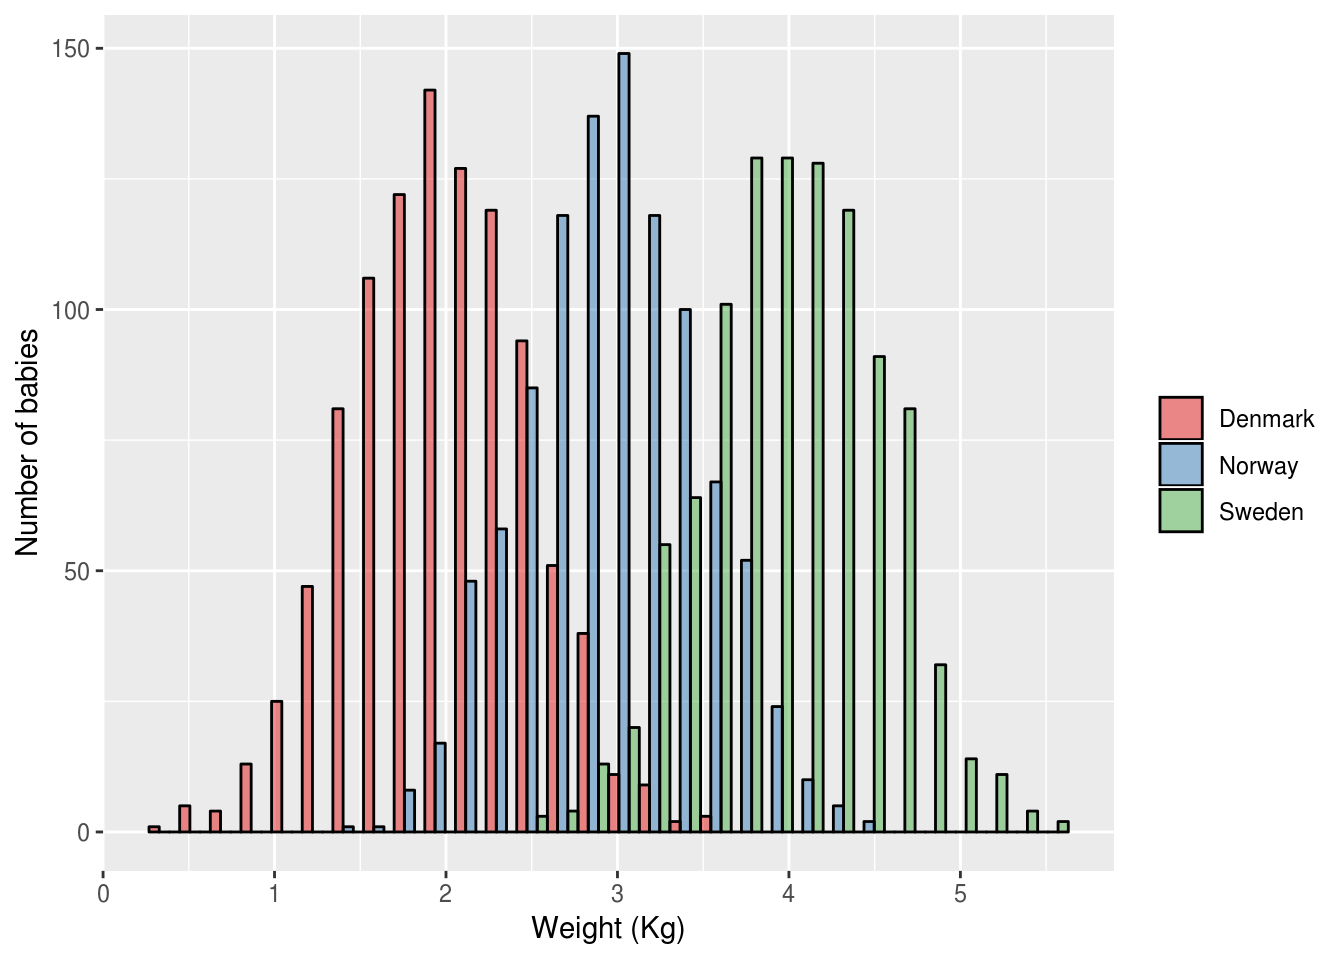
\includegraphics{website_files/figure-latex/unnamed-chunk-24-1.pdf}

\newpage

\textbf{Linear regression}:

\(\rightarrow\) Testing if the effect of country on average birth weight
(continuous outcome) is different than zero

\[\text{birth weight} = \beta_0 + \beta_1 \times \text{is Norway} + \beta_2 \times \text{is Denmark} + \text{error}\]
\[\text{H}_0: \beta_1 = \beta_2 = 0\]
\[\text{H}_1: \beta_1 \ne 0 \text{ and/or } \beta_2 \ne 0\]

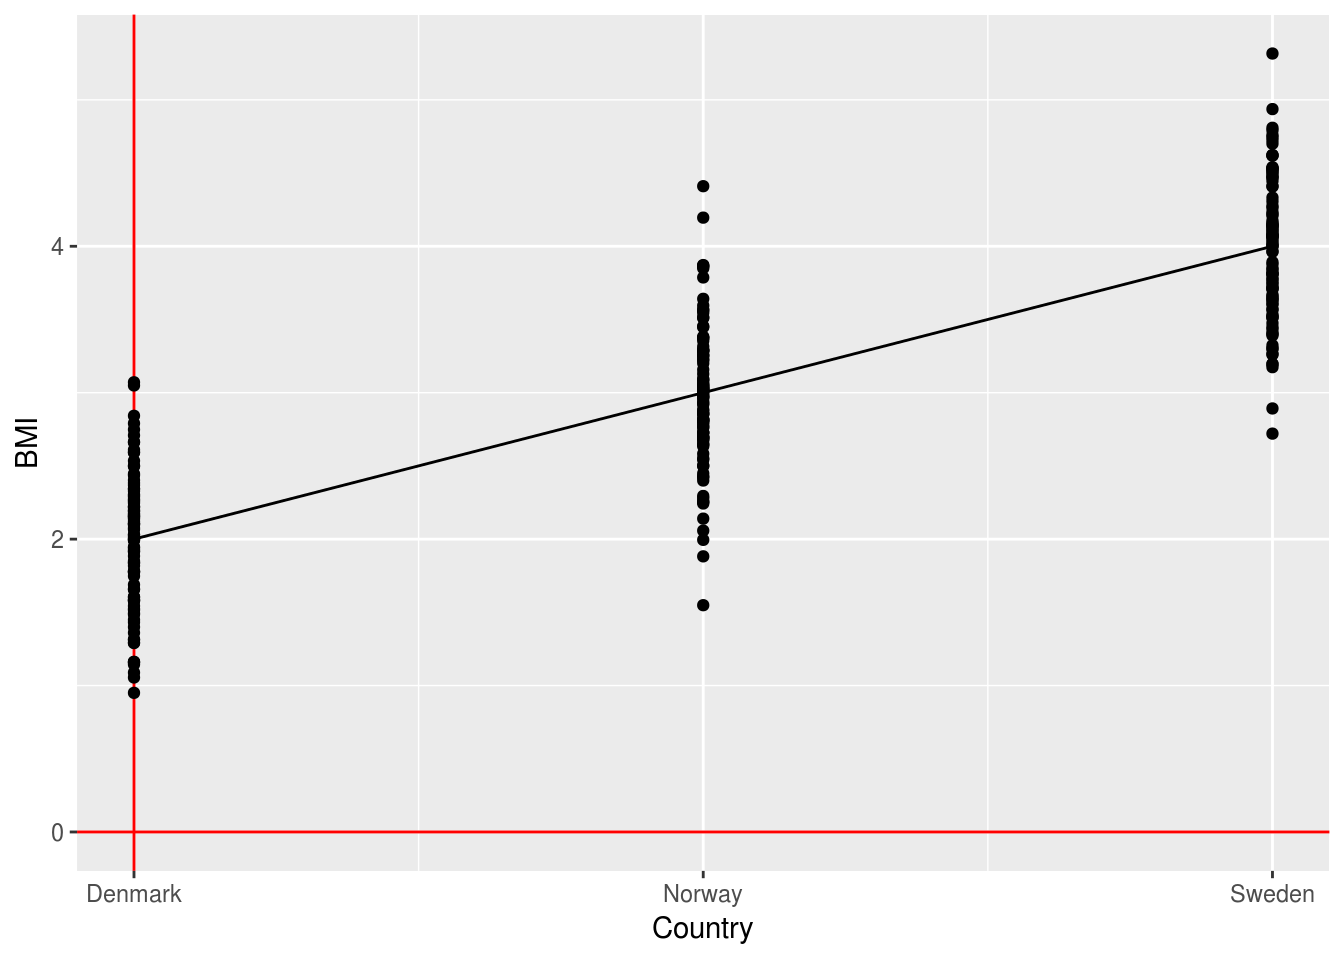
\includegraphics{website_files/figure-latex/unnamed-chunk-25-1.pdf}

\textbf{Conclusion}:

\begin{itemize}
\tightlist
\item
  ANOVA is a linear regression with a categorical exposure
\end{itemize}

\newpage

\subsubsection{Example 2}\label{example-2-6}

\textbf{ANOVA}:

\(\rightarrow\) \hfill \break
\hfill \break
\hfill \break
\(H_0:\) \hfill \break
\hfill \break
\hfill \break
\(H_1:\) \hfill \break
\hfill \break
\hfill \break

\textbf{Linear regression}:

\(\rightarrow\) \hfill \break
\hfill \break
\hfill \break
\hfill \break
\hfill \break
\hfill \break
\(H_0:\) \hfill \break
\hfill \break
\hfill \break
\(H_1:\) \hfill \break
\hfill \break
\hfill \break

\subsection{Logistic regression
models}\label{logistic-regression-models}

Logistic regression is essentially the same as linear regression, but it
is used when:

\begin{itemize}
\tightlist
\item
  You have a binary (0/1) outcome
\item
  You are doing a case-control study {[}case control studies can ONLY be
  analysed using logistic regression{]}
\end{itemize}

\subsubsection{Aim/Outcome/Exposure/Parametric/Dependencies}\label{aimoutcomeexposureparametricdependencies-6}

\textbf{Aim}: Hypothesis testing and estimating the effect size of the
association between outcome and exposure

\textbf{Outcome}: \emph{Binary variable}

\textbf{Exposure}: Continuous, Binary, Categorical, Count variable

\textbf{Parametric assumptions}: No

\textbf{Dependencies}: None (all observations independent)

\subsubsection{Example 1}\label{example-1-7}

\(\rightarrow\) Testing if percentage of women (binary outcome) differ
across the bydels of Oslo (categorical exposure)

\[\text{log}\left(\frac{\text{Pr(Is woman)}}{\text{Pr(Is man)}}\right) = \beta_0 + \beta_1 \times \text{bydel}_1 + \beta_2 \times \text{bydel}_2 + \beta_3 \times \text{bydel}_3 + \text{error}\]

\[\text{H}_0: \beta_1 = \beta_2 = \beta_3 = 0\]
\[\text{H}_1: \beta_1 \ne 0 \text{and/or} \beta_2 \ne 0 \text{and/or} \beta_3 \ne 0\]

\subsubsection{Example 2}\label{example-2-7}

\(\rightarrow\) Testing if risk of unemployment (binary outcome) is
associated with parents' income (continuous exposure)

\[\text{log}\left(\frac{\text{Pr(Is unemployed)}}{\text{Pr(Is employed)}}\right) = \beta_0 + \beta_1 \times \text{parent's income} + \text{error}\]

\[\text{H}_0: \beta_1 = 0\] \[\text{H}_1: \beta_1 \ne 0\]

\subsubsection{Example 3}\label{example-3-6}

\(\rightarrow\) Testing if risk of smoking (binary outcome) is
associated with parents' smoking status (binary exposure)

\[\text{log}\left(\frac{\text{Pr(Is smoker)}}{\text{Pr(Is not smoker)}}\right) = \beta_0 + \beta_1 \times \text{parent's are smokers} + \text{error}\]

\[\text{H}_0: \beta_1 = 0\] \[\text{H}_1: \beta_1 \ne 0\]

\subsubsection{Example 4}\label{example-4-5}

\(\rightarrow\) \hfill \break
\hfill \break
\hfill \break
\hfill \break
\hfill \break
\hfill \break
\(H_0:\) \hfill \break
\hfill \break
\hfill \break
\(H_1:\)

\subsubsection{Example 5}\label{example-5-1}

\(\rightarrow\) \hfill \break
\hfill \break
\hfill \break
\hfill \break
\hfill \break
\hfill \break
\(H_0:\) \hfill \break
\hfill \break
\hfill \break
\(H_1:\)

\newpage

\subsection{Poisson/negative-binomial regression
models}\label{poissonnegative-binomial-regression-models}

Poisson/negative-binomial regression is essentially the same as linear
regression, but it is used when:

\begin{itemize}
\tightlist
\item
  You have a count outcome
\end{itemize}

Negative-binomial regression is a more flexible version of poisson
regression. Poisson regression requires that the residual variation
(after fitting the model) is equal to the expected mean. This is quite
often not the case. Negative-binomial regression fits the variation and
the mean separately, removing this problem. It is therefore recommended
that you always use a negative-binomial regression instead of a poisson
regression. The only exception is if you encounter statistical errors
with the negative-binomial regression (i.e.~it won't converge/run), then
a poisson regression is your only option.

\subsubsection{Aim/Outcome/Exposure/Parametric/Dependencies}\label{aimoutcomeexposureparametricdependencies-7}

\textbf{Aim}: Hypothesis testing and estimating the effect size of the
association between outcome and exposure

\textbf{Outcome}: \emph{Count variable}

\textbf{Exposure}: Continuous, Binary, Categorical, Count variable

\textbf{Parametric assumptions for Poisson}: Mean equals variable

\textbf{Parametric assumptions for negative-binomial}: No

\textbf{Dependencies}: None (all observations independent)

\subsubsection{Example 1}\label{example-1-8}

\(\rightarrow\) Testing if average number of influenza cases (count
outcome) is different between 2000-2009 and 2010-2015 (binary exposure)
in Norway

\[\text{yearly number of influenza cases} = \beta_0 + \beta_1 \times \text{is 2010 to 2015} + \text{error}\]

\[\text{H}_0: \beta_1 = 0\] \[\text{H}_1: \beta_1 \ne 0\]

\subsubsection{Example 2}\label{example-2-8}

\(\rightarrow\) \hfill \break
\hfill \break
\hfill \break
\hfill \break
\hfill \break
\hfill \break
\(H_0:\) \hfill \break
\hfill \break
\hfill \break
\(H_1:\)

\newpage

\subsection{Cox regression models}\label{cox-regression-models}

Cox regression models should be used when your outcome is
``time-to-event''.

The most common example of this is when you are following a cohort of
people over time, trying to observe an (e.g.~sickness, death, response).
Your outcome is ``length of time until person X gets disease Y''.
However, a number of your participants stop responding at some point, so
you only know ``person X was healthy up until 200 days, when we lost
contact''.Thus person X's outcome has been censored at day 200.

\subsubsection{Aim/Outcome/Exposure/Parametric/Dependencies}\label{aimoutcomeexposureparametricdependencies-8}

\textbf{Aim}: Hypothesis testing and estimating the effect size of the
association between outcome and exposure

\textbf{Outcome}: \emph{Censored variable} (time-to-event)

\textbf{Exposure}: Continuous, Binary, Categorical, Count variable

\textbf{Parametric assumptions}: Proportional hazards

\textbf{Dependencies}: None (all observations independent)

\subsubsection{Example 1}\label{example-1-9}

\(\rightarrow\) Testing if time-to-death (outcome) is associated with
having a hospital-acquired-infection after hip surgery (binary exposure)

\[\lambda(t | X_i) = \lambda_0(t) \times \text{exp}(\beta_1 \times \text{had HAI})\]

Where \(\lambda(t | X_i)\) is the hazard rate of dying at time \(t\) for
subject \(i\).

\[\text{H}_0: \beta_1 = 0\] \[\text{H}_1: \beta_1 \ne 0\]

\subsubsection{Example 2}\label{example-2-9}

\(\rightarrow\) \hfill \break
\hfill \break
\hfill \break
\hfill \break
\hfill \break
\hfill \break
\(H_0:\) \hfill \break
\hfill \break
\hfill \break
\(H_1:\)

\section{Complicated regression}\label{complicated-regression}

\subsection{Dependencies in your data}\label{dependencies-in-your-data}

\subsubsection{What is independent data}\label{what-is-independent-data}

Broadly, having knowledge about one observation should not give you
knowledge about other observations in your dataset.

For example, if we flip a coin ten times, knowing the result of the
first coin toss (heads) will not give us knowledge about the subsequent
9 coin tosses.

\subsubsection{What is data with
dependencies}\label{what-is-data-with-dependencies}

In reality, most data have dependencies, so we will focus on some of the
most important kinds that will severely impact your analyses if you do
not identify them.

\subsubsection{Repeated measures/longitudinal
data}\label{repeated-measureslongitudinal-data}

If you have a dataset with repeated measures (e.g.~some people in your
cohort have more than one observation), then the repeated observations
on each person cause dependencies in the data. That is, if a person has
their weight measured five times, then just by knowing their first
weight you can have a good guess at what their subsequent weights will
be.

\subsubsection{Matched data}\label{matched-data}

Inside case-control studies, for each case a control (or multiple cases)
can be selected to have similar attributes. For example, for each case,
a control can be selected with a similar age. These controls have been
``matched'' to a case, and have introduced dependencies into the data.

\subsubsection{Grouped/clustered data}\label{groupedclustered-data}

Repeated measures data is a type of clustered data, where each person is
their own cluster. Matched data is also a type of clustered data, where
each group of matched controls-to-a-case is a cluster.

There can be many other kinds of clusters, for example:

\begin{itemize}
\tightlist
\item
  Data sampled from multiple hospitals could have the hospital as the
  cluster variable
\item
  Data sampled from multiple countries could have the country as the
  cluster variable
\item
  Data sampled from multiple counties/municipalities could have the
  country/municipality as the cluster variable
\item
  If it is a study of children, and multiple children from each mother
  are included, then the mother could be the cluster variable
\end{itemize}

\subsection{Analysing data with
dependencies}\label{analysing-data-with-dependencies}

\subsubsection{Mixed effects regression}\label{mixed-effects-regression}

Mixed effects regression is an extension of the simple regression models
(fixed effects) that we learned about in the previous chapter. You can
have:

\begin{itemize}
\tightlist
\item
  Mixed effects linear regression
\item
  Mixed effects logistic regression
\item
  Mixed effects negative-binomial regression
\end{itemize}

Mixed effects models are models that have both fixed and random effects.
``Effects'' is the term used to describe the estimated impact a variable
has on the outcome. For example, ``the effect of smoking on the risk of
lung cancer''.

To determine if an effect is fixed or random, we introduce the concept
of pooling data (i.e.~sharing strength). Let us assume we have sampled
100 people per city for 9 cities, and 2 people for 1 city, and we want
to estimate the average height in each city, we can do one of the
following three options:

\begin{enumerate}
\def\labelenumi{\arabic{enumi}.}
\tightlist
\item
  Within each city, take the average height of the 100 (or 2) sampled
  people (zero pooling)
\item
  Take the average height of 1000 sampled people and say each city is
  the same height (complete pooling)
\item
  Estimate how much the average height varies between the cities. If the
  average height doesn't vary much, give estimates close to \#2. If the
  average height varies a lot, give estimates close to \#1 (partial
  pooling)
\end{enumerate}

Zero pooling tends to work well when you have a limited amount of
effects you want to estimate, each with a good sample size (i.e.~you
don't need to borrow strength from other data points). Partial pooling
tends to work well when you have a large number of effects you want to
estimate, each with a small sample size (i.e.~you need to borrow
strength from other data points).

Fixed effects are estimated with zero pooling. Random effects are
estimated with partial pooling.

With data that has a large number of clusters, the clustering need to be
accounted for in the regression model. This is done by introducing a
variable that uniquely identifies each cluster, and allows the cluster
effect to be estimated (e.g.~in Oslo people are 1\% more likely to die
than in the rest of Norway). If there are a large number of clusters
with a small amount of people in each cluster, then the cluster variable
should be estimated using partial pooling (i.e.~random effects).

In summary: Mixed effects regression should be used for
grouped/clustered/matched data (and subsequently repeated
measures/longitudinal data).

\subsubsection{Conditional logistic
regression}\label{conditional-logistic-regression}

Conditional logistic regression can also be used for matched data with a
binary outcome, however, it is less flexible than mixed effects
regression.

\subsection{(TBD) Understanding the best practices for data files and
project
folders}\label{tbd-understanding-the-best-practices-for-data-files-and-project-folders}

\section{Good folder structure}\label{good-folder-structure}

\subsection{Data and results}\label{data-and-results}

\begin{itemize}
\tightlist
\item
  One folder for raw data
\item
  One folder for temporary data (if needed)
\item
  One folder for clean data
\end{itemize}

\begin{figure}
\centering
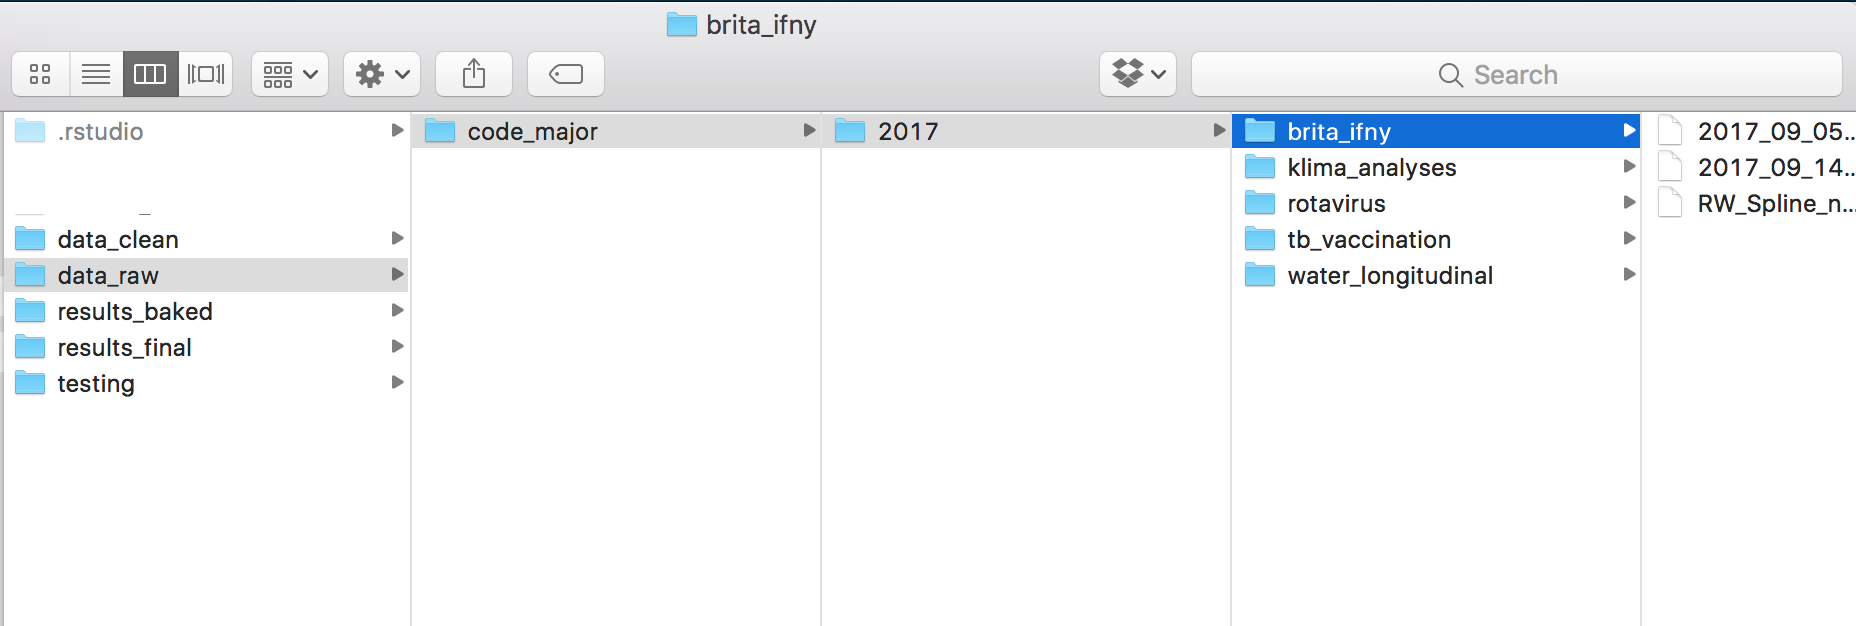
\includegraphics{resources/folder_raw.png}
\caption{img}
\end{figure}

\begin{itemize}
\tightlist
\item
  One folder for shared results (dropbox)
\item
  Every time you run your analyses, you should store your new results in
  a new day's folder, allowing you to always access your previous
  results
\item
  Labelling by date (year-month-day) is a lot more intuitive than
  ``results\_1'', ``results\_2'', ``results\_final'',
  ``results\_final\_final''
\item
  Label in the format 2017-09-01 so that your computer can easily sort
  the results (the padding/leading 0s are important for sorting!)
\item
  Do not label folders using the format 2017-SEP-1 (it doesn't sort
  well)
\item
  Do not label folders using the format 1-SEP-17 (it doesn't sort well)
\end{itemize}

\begin{figure}
\centering
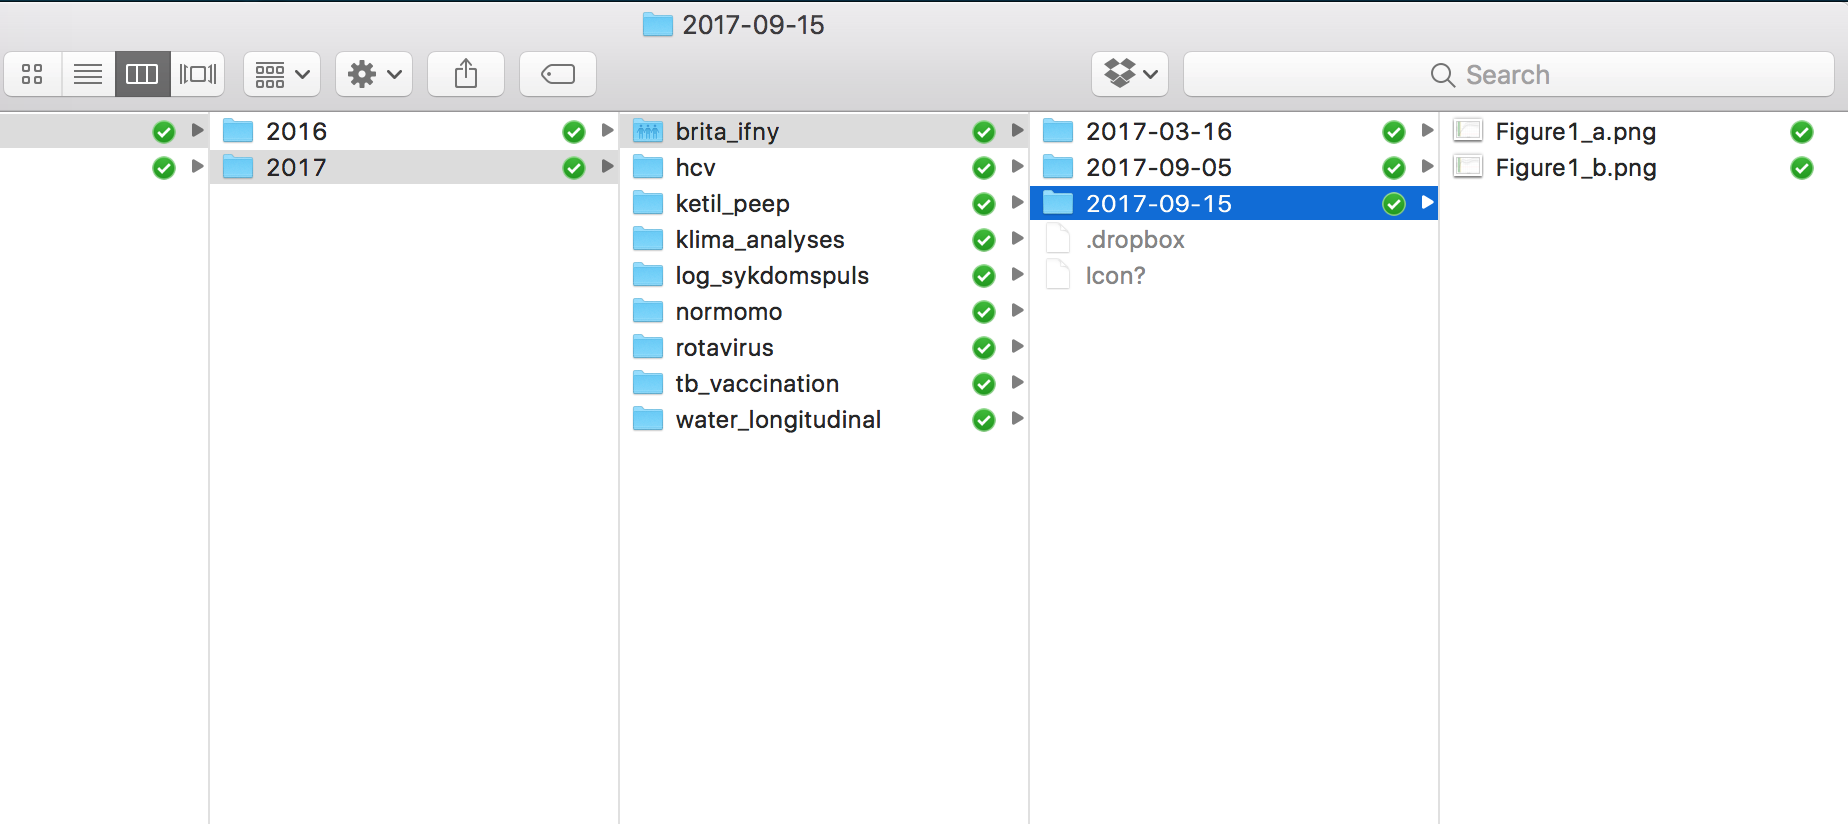
\includegraphics{resources/folder_shared.png}
\caption{img}
\end{figure}

\subsection{Keep your source code separate from
data}\label{keep-your-source-code-separate-from-data}

Source code is:

\begin{itemize}
\tightlist
\item
  Not sensitive
\item
  Very easy to accidentally delete and/or overwrite
\end{itemize}

This means it is perfect to be uploaded to \url{http://github.com} where
you can store every version of your code, and never have to worry about
losing an old copy

\begin{figure}
\centering
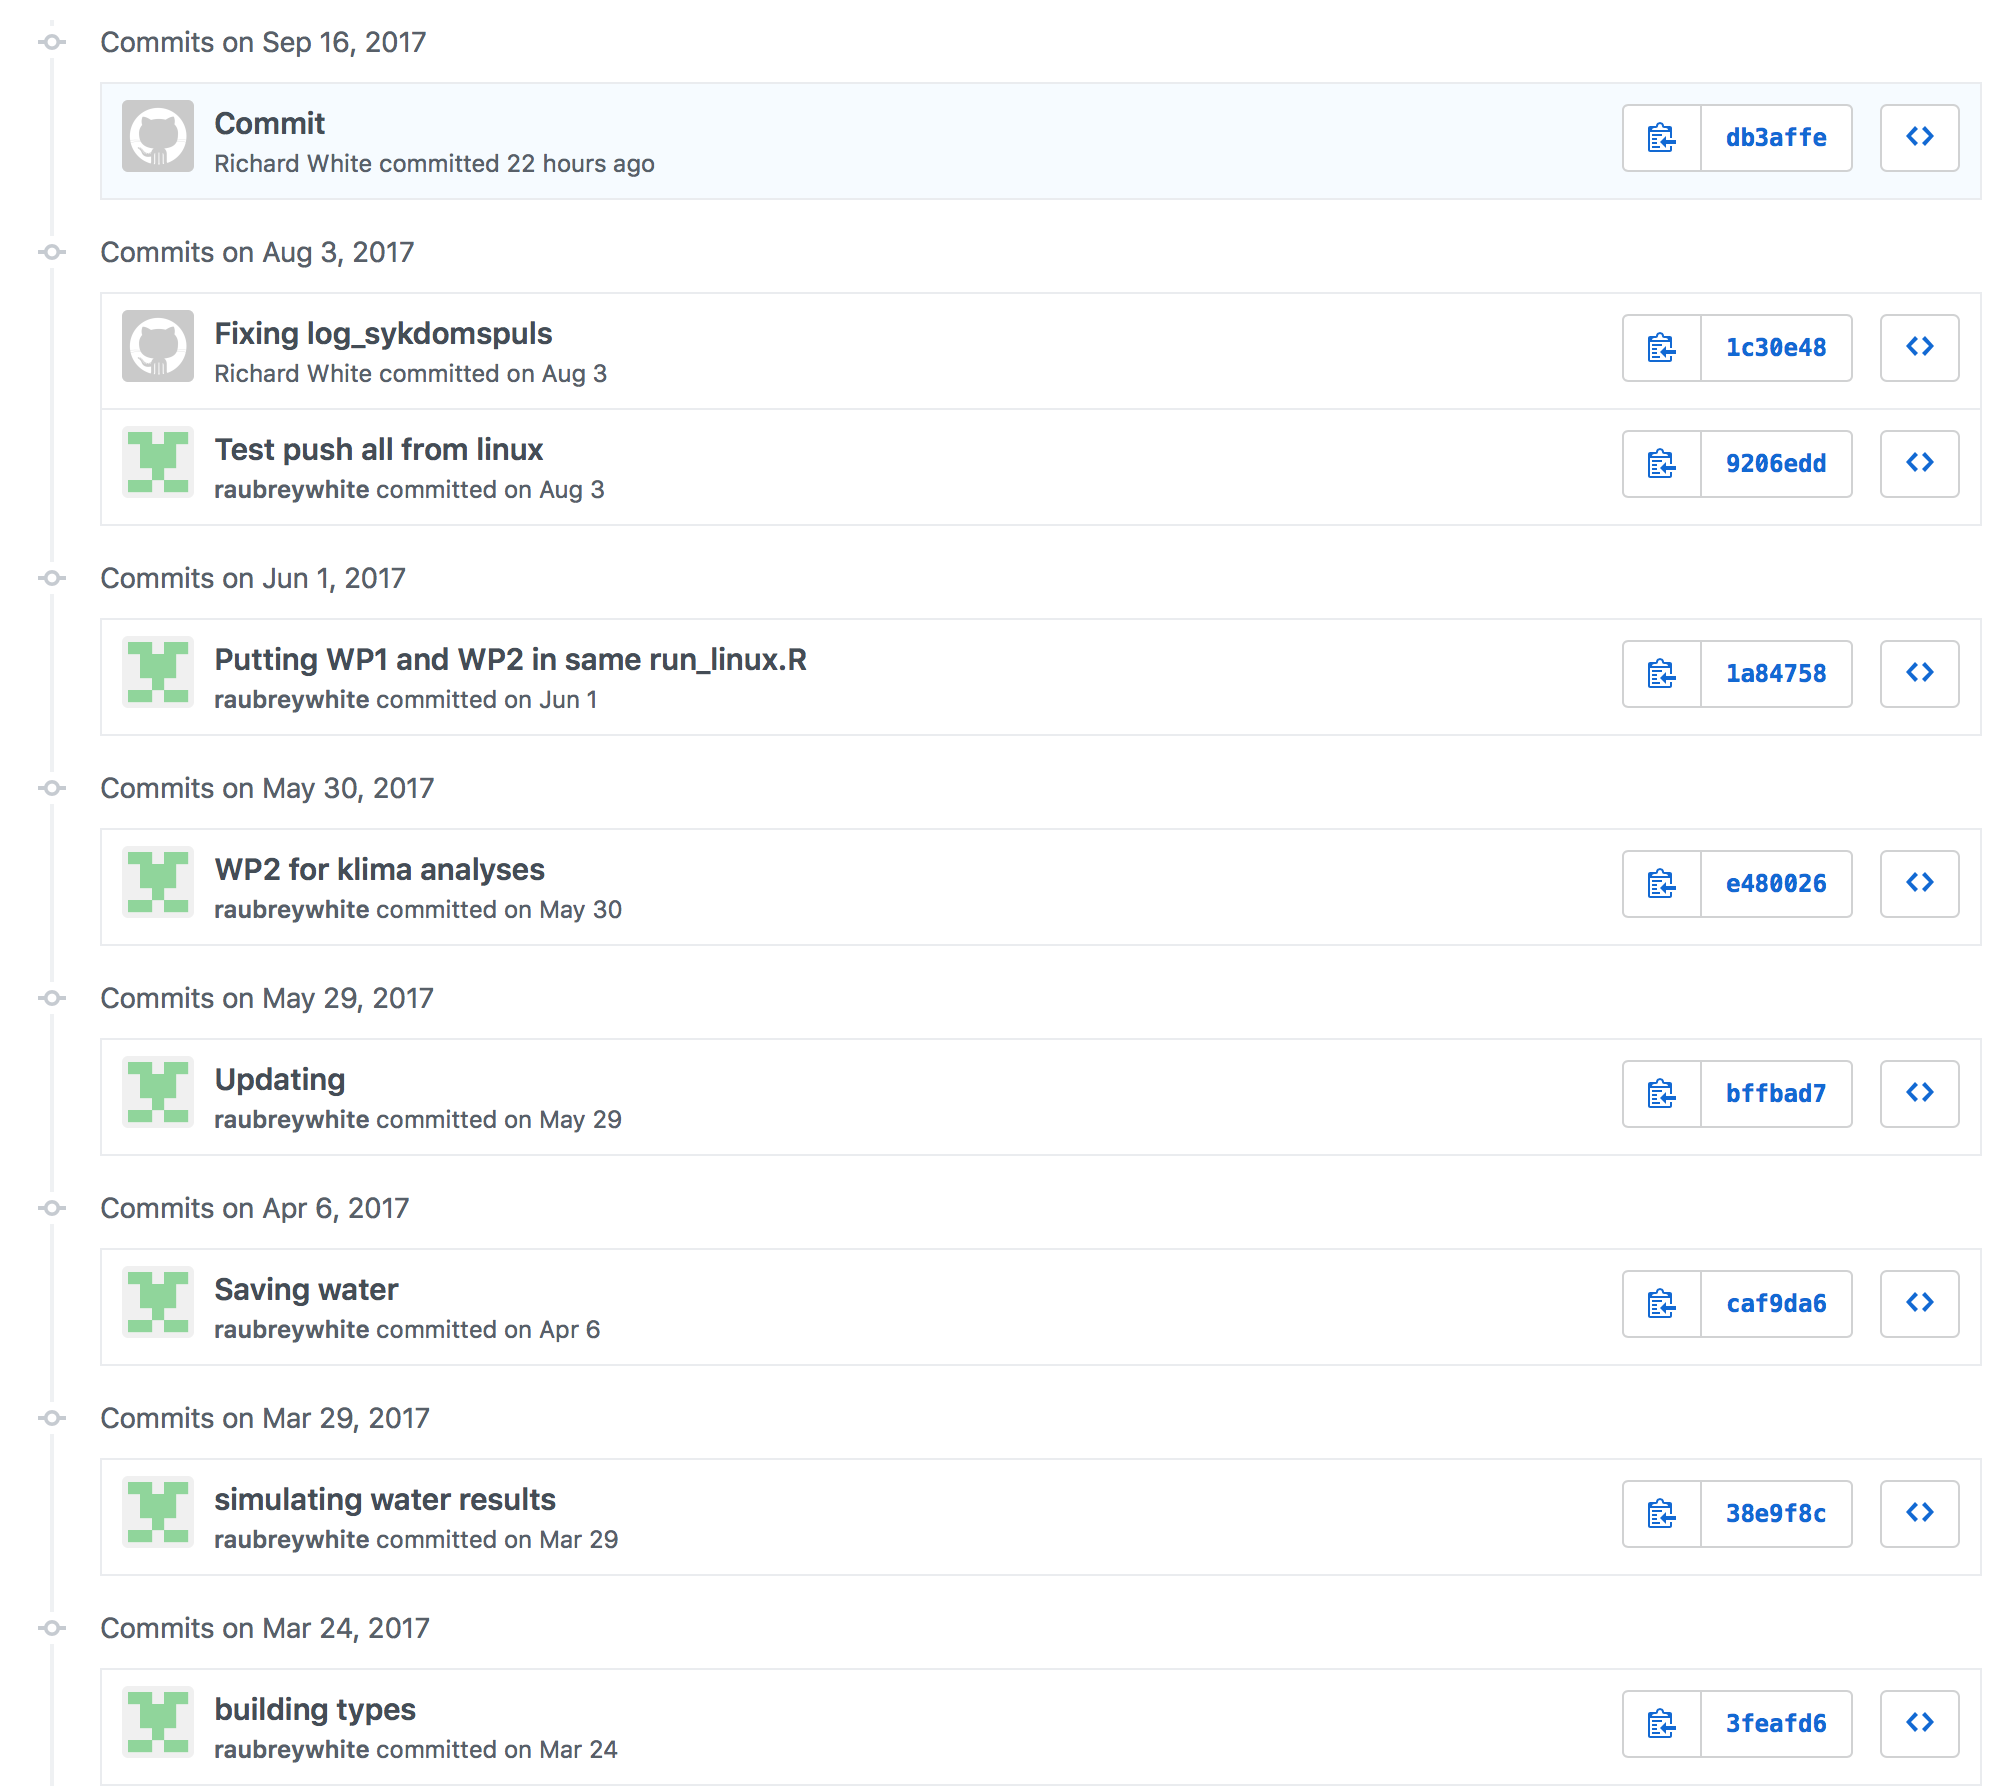
\includegraphics{resources/git_commit.png}
\caption{img}
\end{figure}

You can also see the differences between your versions:

\begin{figure}
\centering
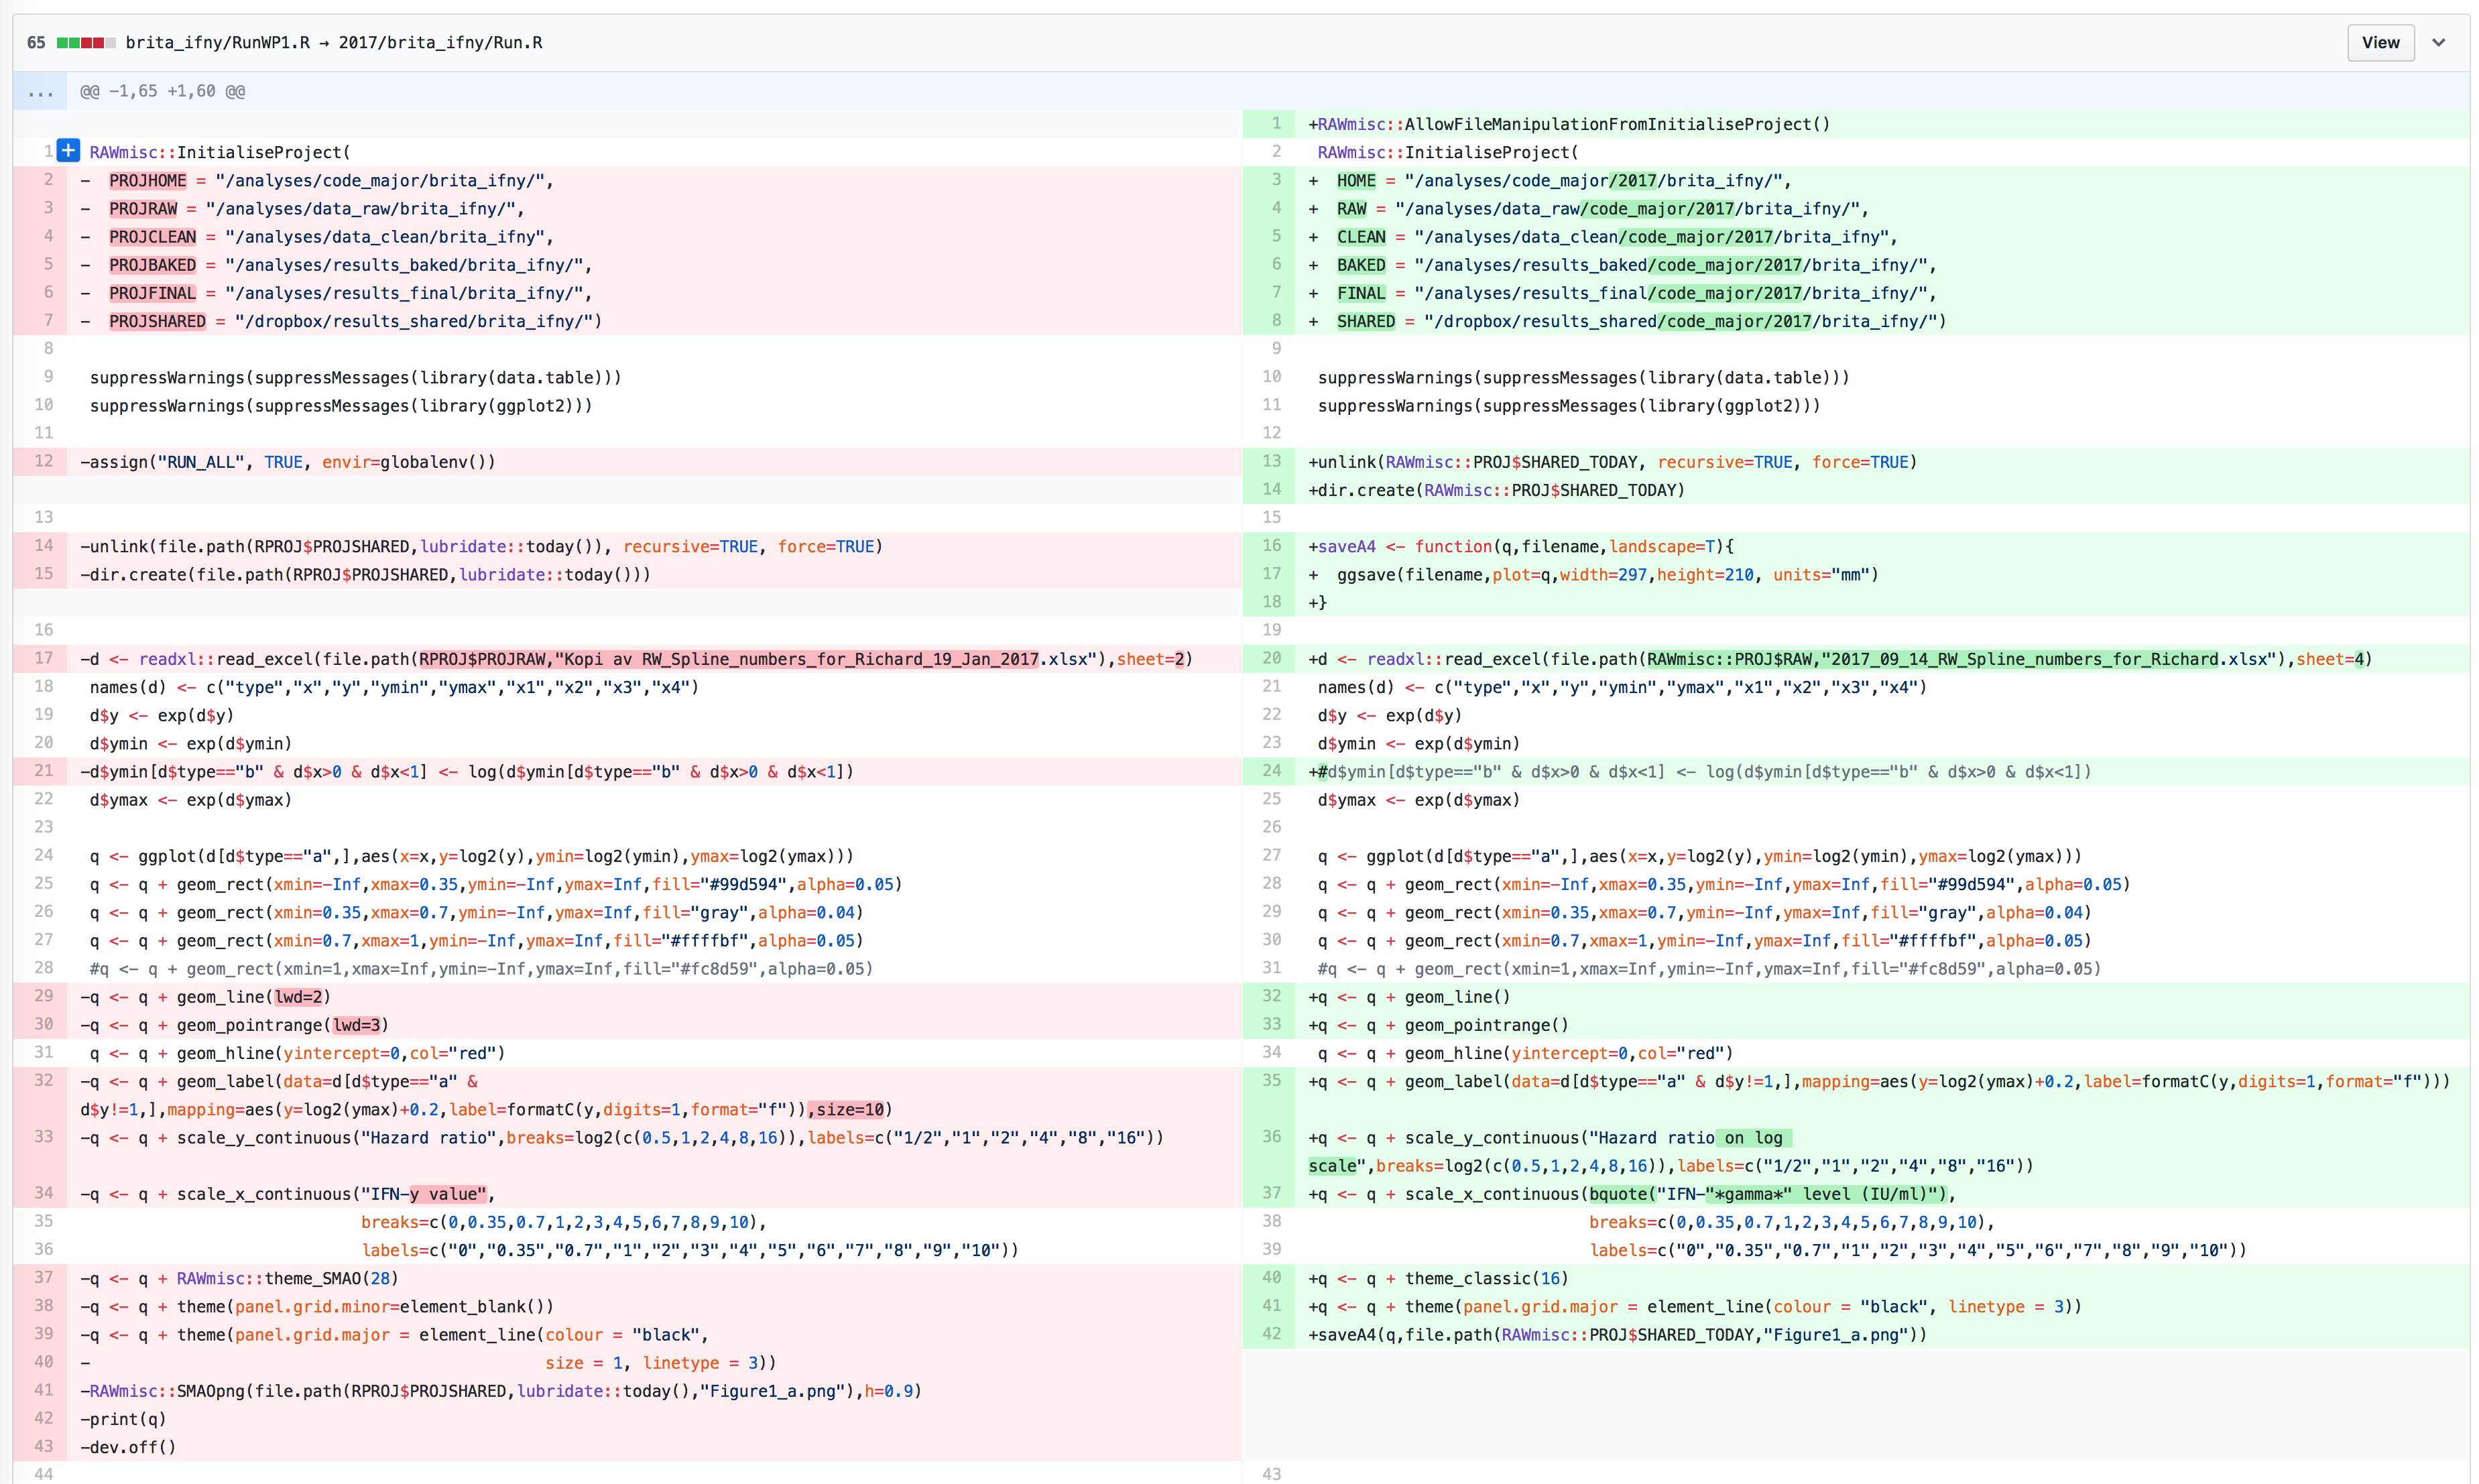
\includegraphics{resources/git_changes.png}
\caption{img}
\end{figure}

It is best to keep each project in it's own folder. Within each folder,
there should be a masterfile (``Run'') that will perform all of the
necessary tasks in the entire analysis:

\begin{itemize}
\tightlist
\item
  Clean data
\item
  Run analyses
\end{itemize}

\begin{figure}
\centering
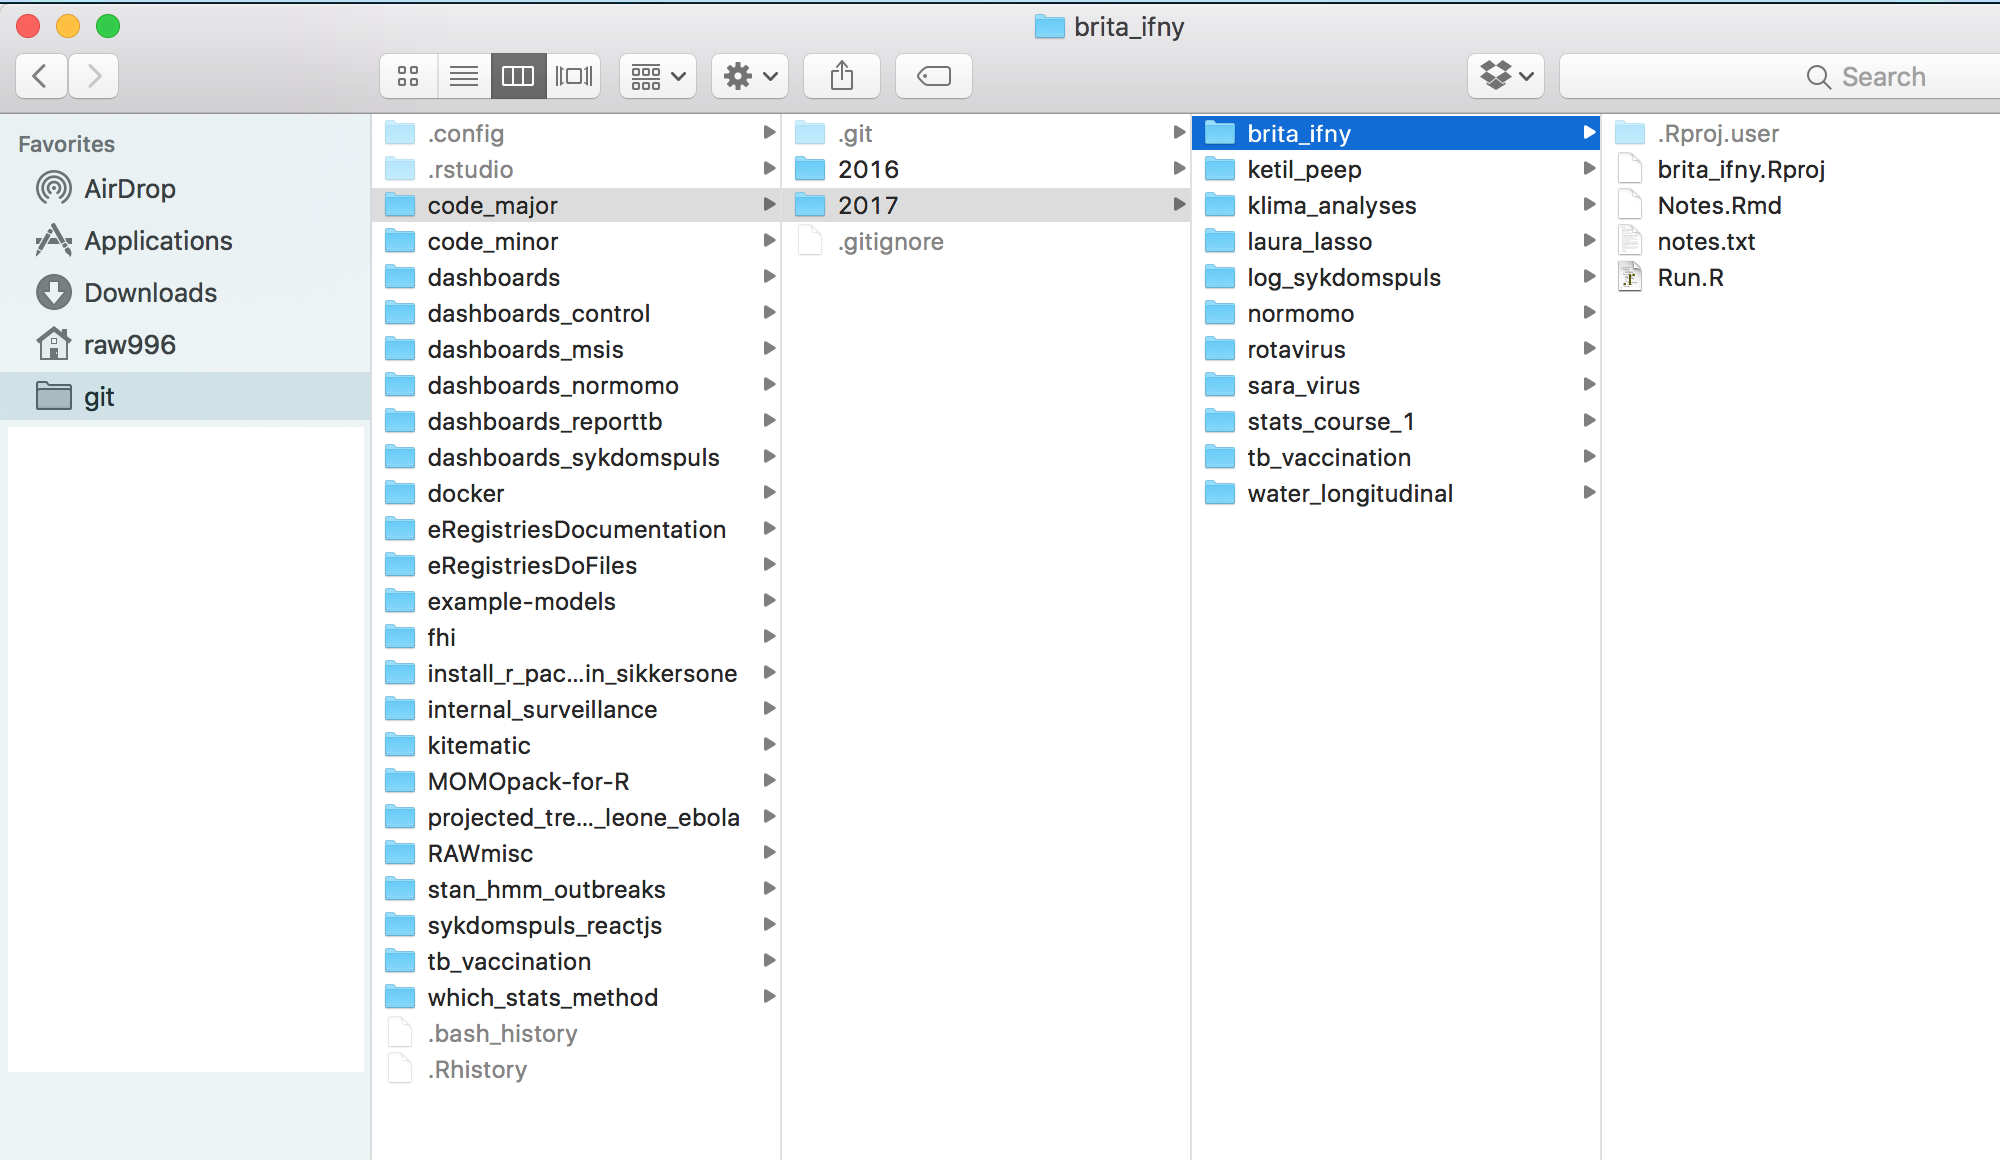
\includegraphics{resources/folder_git.png}
\caption{img}
\end{figure}

Do files/scripts should be numbered:

\begin{itemize}
\tightlist
\item
  0\_run\_all.do
\item
  1\_clean\_lab\_data.do
\item
  2\_clean\_lifestyle\_data.do
\item
  3\_merge\_lab\_lifestyle\_data.do
\item
  4\_descriptive\_analyses.do
\item
  5\_regression\_analyses.do
\end{itemize}

It is very very very important that analysis files only use the
``clean'' data (from the clean data folder), and perform ZERO changes to
the data. All necessary changes and/or variable creations must be done
in the data cleaning do files.

\section{Examples}\label{examples-1}

\subsection{Poisons Information
Center}\label{poisons-information-center}

\begin{figure}
\centering
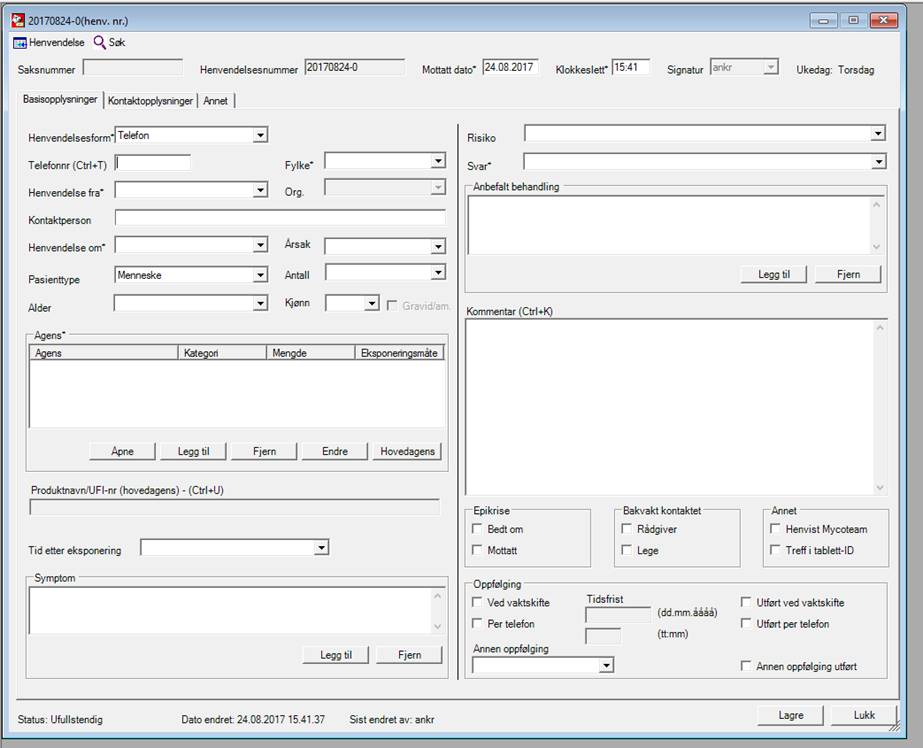
\includegraphics{resources/poisons_information_center.jpg}
\caption{img}
\end{figure}

Scenario:

\begin{itemize}
\tightlist
\item
  Approximately 40 000 calls per year
\item
  The frequency of calls regarding different drugs/plants etc varies
  greatly, from a couple per year to thousands per year, so most
  probably one method will not cover everything.
\item
  The registration of data is done while on the phone, and we know there
  are mistakes
\item
  Only the field Kommentar has free text
\end{itemize}

Question: Is the number of calls regarding women aged 15-19 who have
been exposed to paracetamol rising or falling over the years.

\textbf{Aim}:

\textbf{Outcome}:

\textbf{Exposure}:

\textbf{Parametric assumptions}:

\textbf{Dependencies}:

\subsection{Norwegian Water Pipes}\label{norwegian-water-pipes}

Scenario:

\begin{itemize}
\tightlist
\item
  146 waterworks in 19 counties in Norway
\item
  Each waterwork uses pipes to deliver water to households
\item
  Information on each waterwork:
\item
  Length of pipes made out of asbestos (in meters)
\item
  Length of pipes made out of iron/steel (in meters)
\item
  Length of pipes made out of PVC (in meters)
\item
  Length of pipes made out of PE/PEH (in meters)
\item
  Length of pipes made out of other (in meters)
\item
  Length of pipes made out of unknown (in meters)
\item
  Length of pipes installed before 1910 (in meters)
\item
  Length of pipes installed in 1910-1940 (in meters)
\item
  Length of pipes installed in 1941-1970 (in meters)
\item
  Length of pipes installed in 1971-2000 (in meters)
\item
  Length of pipes installed after 2000 (in meters)
\item
  Length of pipes installed during an unknown period (in meters)
\item
  Each year, some new pipes are laid to extend the network
\item
  Each year, some pipes are replaced
\item
  Interruption in water delivery is estimated in hours per calendar year
\item
  Data is only for 2015
\end{itemize}

Question: Is there an association between ``interuption in water
delivery'' and ``type of pipe material'' and ``pipe installation
period''

\textbf{Aim}:

\textbf{Outcome}:

\textbf{Exposure}:

\textbf{Parametric assumptions}:

\textbf{Dependencies}:

\subsection{Early warning system (EWS) for waterborne outbreaks (part
1)}\label{early-warning-system-ews-for-waterborne-outbreaks-part-1}

Scenario:

\begin{itemize}
\tightlist
\item
  NorSySS is a syndromic surveillance system for infectious diseases,
  run by the NIPH.
\item
  The system is based on national ICPC coded consultation data from
  general practice in Norway.
\item
  We want to study to what extent NorSySS can serve as an early warning
  system for local waterborne outbreaks by alerting us to increases in
  consultation rates for syndromes indicative of gastrointestinal
  diseases.\\
\item
  Retrospective syndrome data (number of gastritis cases, per week, for
  each municipality) from NorSySS will be aligned with outbreak data
  (outbreak=yes/no) from the national web-based outbreak rapid alert
  system (Vesuv) for the period 2006-2017.
\end{itemize}

Question: Is there an association between ``recorded outbreak'' and
``number of gastritis cases''

\textbf{Aim}:

\textbf{Outcome}:

\textbf{Exposure}:

\textbf{Parametric assumptions}:

\textbf{Dependencies}:

\subsection{Early warning system (EWS) for waterborne outbreaks (part
2)}\label{early-warning-system-ews-for-waterborne-outbreaks-part-2}

Scenario:

\begin{itemize}
\tightlist
\item
  We have weekly data on water quality from water works (e.g.~pH,
  turbidity)
\item
  We have weekly number of gastritis cases, per week, for each
  municipality
\item
  We hope to increase the knowledge about causes of waterborne outbreaks
  and to develop an improved surveillance system for early detection of
  future outbreaks.
\end{itemize}

Question: Is there an association between ``weekly number of gastritis
cases'' and ``water quality from the water works''

\textbf{Aim}:

\textbf{Outcome}:

\textbf{Exposure}:

\textbf{Parametric assumptions}:

\textbf{Dependencies}:

\subsection{Incidents in the water supply system and
illness}\label{incidents-in-the-water-supply-system-and-illness}

Scenario:

\begin{itemize}
\tightlist
\item
  Data from the water works operation (pH, turbidity) will be linked to
  health outcome among recipients of the drinking water.
\item
  The study will be a prospective cohort study, with data collected
  among a random selection of water works.
\item
  Data from the recruited water works will be collected in the period
  autumn 2017 and the 12 following months.
\item
  Approximately 350 water works will be recruited to provide monthly
  data on hygienic critical points related to operation and maintenance
  of the water supply system.
\item
  In parallel, a cohort of approximately 9000 persons, served by water
  from the recruited water works, will submit monthly reports on
  symptoms that may indicate gastrointestinal illness.
\item
  The data collection will start in the autumn of 2017 and continue for
  12 months.
\end{itemize}

Question: Is water quality a risk factor for getting sick?

\textbf{Aim}:

\textbf{Outcome}:

\textbf{Exposure}:

\textbf{Parametric assumptions}:

\textbf{Dependencies}:

\subsection{Compliance with boil water advisories and perception of
risks}\label{compliance-with-boil-water-advisories-and-perception-of-risks}

Scenario:

\begin{itemize}
\tightlist
\item
  In this study, the compliance and perception of risks among the public
  with boil water advisories (BWAs) will be examined.
\item
  Although BWAs is a common practice among water utilities, a meta-study
  suggest that there is limited information and studies on the
  compliance of BWAs.
\item
  This part, the compliance and perception of risks will be done by
  studying the perception of and adherence to BWAs among the consumers
  of drinking water in Bærum municipality.
\item
  Even though the drinking water in Bærum is considered to have good
  quality, Bærum -- like many water works -- experience situations of
  pressure drops due to breaks and maintenance.
\item
  Research has shown that these situations may lead to an increased risk
  of gastrointestinal infections, and due to this the municipality of
  Bærum has issued a precautionary BWAs to the affected consumers with
  every water outage during the last 5-6 years.
\item
  Every year, some 12,000-22,000 consumers have received a precautionary
  BWA.
\item
  The purpose of these precautionary BWAs is to prevent health
  consequences caused by possible contamination of water. However, we
  know little about the consumer's knowledge about why they receive
  these BWAs, as well as the way the consumers perceive and adhere to
  these BWAs.
\item
  This is a cross-sectional study.
\item
  A web-survey will be presented to a randomly selected sample of
  consumers who received a BWA i Bærum in 2017.
\item
  The web-survey asks about adherence (yes/no) and demographics
  (e.g.~age, sex, income)
\end{itemize}

Question: Estimate adherence by demographics (and identify if it differs
by demographics)

\textbf{Aim}:

\textbf{Outcome}:

\textbf{Exposure}:

\textbf{Parametric assumptions}:

\textbf{Dependencies}:

\section{Solutions}\label{solutions}

\subsection{Poisons Information
Center}\label{poisons-information-center-1}

Scenario:

\begin{itemize}
\tightlist
\item
  Approximately 40 000 calls per year
\item
  The frequency of calls regarding different drugs/plants etc varies
  greatly, from a couple per year to thousands per year, so most
  probably one method will not cover everything.
\item
  The registration of data is done while on the phone, and we know there
  are mistakes
\item
  Only the field Kommentar has free text
\end{itemize}

Question: Is the number of calls regarding women aged 15-19 who have
been exposed to paracetamol rising or falling over the years.

\textbf{Aim}: Hypothesis testing (maybe estimation of yearly effect)

\textbf{Outcome}: Count data (number of calls regarding women aged 15-19
who have been exposed to paracetamol)

\textbf{Exposure}: Continuous (year)

\textbf{Parametric assumptions}: None

\textbf{Dependencies}: None

\textbf{Appropriate Method}: Negative-binomial regression

\textbf{Example STATA code}:

\begin{verbatim}
nbreg number_of_calls year
\end{verbatim}

\subsection{Norwegian Water Pipes}\label{norwegian-water-pipes-1}

Scenario:

\begin{itemize}
\tightlist
\item
  146 waterworks in 19 counties in Norway
\item
  Each waterwork uses pipes to deliver water to households
\item
  Information on each waterwork:
\item
  Length of pipes made out of asbestos (in meters)
\item
  Length of pipes made out of iron/steel (in meters)
\item
  Length of pipes made out of PVC (in meters)
\item
  Length of pipes made out of PE/PEH (in meters)
\item
  Length of pipes made out of other (in meters)
\item
  Length of pipes made out of unknown (in meters)
\item
  Length of pipes installed before 1910 (in meters)
\item
  Length of pipes installed in 1910-1940 (in meters)
\item
  Length of pipes installed in 1941-1970 (in meters)
\item
  Length of pipes installed in 1971-2000 (in meters)
\item
  Length of pipes installed after 2000 (in meters)
\item
  Length of pipes installed during an unknown period (in meters)
\item
  Each year, some new pipes are laid to extend the network
\item
  Each year, some pipes are replaced
\item
  Interruption in water delivery is estimated in hours per calendar year
\item
  Data is only for 2015
\end{itemize}

Question: Is there an association between ``interuption in water
delivery'' and ``type of pipe material'' and ``pipe installation
period''

\textbf{Aim}: Hypothesis testing

\textbf{Outcome}: Count (hours interruption in water delivery)

\textbf{Exposure}: 12 continuous variables

\textbf{Parametric assumptions}: None

\textbf{Dependencies}: No

\textbf{Appropriate Method}: Negative-binomial regression

\textbf{Example STATA code}:

\begin{verbatim}
nbreg hoursInterrupted pipesAsbestos pipesIronSteel pipesPVC ... pipes1910 ...
\end{verbatim}

\subsection{Early warning system (EWS) for waterborne outbreaks (part
1)}\label{early-warning-system-ews-for-waterborne-outbreaks-part-1-1}

Scenario:

\begin{itemize}
\tightlist
\item
  NorSySS is a syndromic surveillance system for infectious diseases,
  run by the NIPH.
\item
  The system is based on national ICPC coded consultation data from
  general practice in Norway.
\item
  We want to study to what extent NorSySS can serve as an early warning
  system for local waterborne outbreaks by alerting us to increases in
  consultation rates for syndromes indicative of gastrointestinal
  diseases.\\
\item
  Retrospective syndrome data (number of gastritis cases, per week, for
  each municipality) from NorSySS will be aligned with outbreak data
  (outbreak=yes/no) from the national web-based outbreak rapid alert
  system (Vesuv) for the period 2006-2017.
\end{itemize}

Question: Is there an association between ``recorded outbreak'' and
``number of gastritis cases''

\textbf{Aim}: Hypothesis testing

\textbf{Outcome}: Binary (recorded outbreak)

\textbf{Exposure}: Count (number of gastritis cases)

\textbf{Parametric assumptions}: None

\textbf{Dependencies}: Yes (longitudinal data by municipality)

\textbf{Appropriate Method}: Mixed effects logistic regression

\subsection{Early warning system (EWS) for waterborne outbreaks (part
2)}\label{early-warning-system-ews-for-waterborne-outbreaks-part-2-1}

Scenario:

\begin{itemize}
\tightlist
\item
  We have weekly data on water quality from water works (e.g.~pH,
  turbidity)
\item
  We have weekly number of gastritis cases, per week, for each
  municipality
\item
  We hope to increase the knowledge about causes of waterborne outbreaks
  and to develop an improved surveillance system for early detection of
  future outbreaks.
\end{itemize}

Question: Is there an association between ``weekly number of gastritis
cases'' and ``water quality from the water works''

\textbf{Aim}: Hypothesis testing

\textbf{Outcome}: Count (number of gastritis cases)

\textbf{Exposure}: Continuous (pH, turbidity)

\textbf{Parametric assumptions}: None

\textbf{Dependencies}: Yes (longitudinal data by municipality)

\textbf{Appropriate Method}: Mixed effects negative-binomial regression

\subsection{Incidents in the water supply system and
illness}\label{incidents-in-the-water-supply-system-and-illness-1}

Scenario:

\begin{itemize}
\tightlist
\item
  Data from the water works operation (pH, turbidity) will be linked to
  health outcome among recipients of the drinking water.
\item
  The study will be a prospective cohort study, with data collected
  among a random selection of water works.
\item
  Data from the recruited water works will be collected in the period
  autumn 2017 and the 12 following months.
\item
  Approximately 350 water works will be recruited to provide monthly
  data on hygienic critical points related to operation and maintenance
  of the water supply system.
\item
  In parallel, a cohort of approximately 9000 persons, served by water
  from the recruited water works, will submit monthly reports on
  symptoms that may indicate gastrointestinal illness.
\item
  The data collection will start in the autumn of 2017 and continue for
  12 months.
\end{itemize}

Question: Is water quality a risk factor for getting sick?

\textbf{Aim}: Hypothesis testing

\textbf{Outcome}: Binary (sick yes/no)

\textbf{Exposure}: Continuous (pH, turbidity)

\textbf{Parametric assumptions}: None

\textbf{Dependencies}: Yes (longitudinal data by person, clustered by
waterwork and/or municipality)

\textbf{Appropriate Method}: Mixed effects logistic regression

\subsection{Compliance with boil water advisories and perception of
risks}\label{compliance-with-boil-water-advisories-and-perception-of-risks-1}

Scenario:

\begin{itemize}
\tightlist
\item
  In this study, the compliance and perception of risks among the public
  with boil water advisories (BWAs) will be examined.
\item
  Although BWAs is a common practice among water utilities, a meta-study
  suggest that there is limited information and studies on the
  compliance of BWAs.
\item
  This part, the compliance and perception of risks will be done by
  studying the perception of and adherence to BWAs among the consumers
  of drinking water in Bærum municipality.
\item
  Even though the drinking water in Bærum is considered to have good
  quality, Bærum -- like many water works -- experience situations of
  pressure drops due to breaks and maintenance.
\item
  Research has shown that these situations may lead to an increased risk
  of gastrointestinal infections, and due to this the municipality of
  Bærum has issued a precautionary BWAs to the affected consumers with
  every water outage during the last 5-6 years.
\item
  Every year, some 12,000-22,000 consumers have received a precautionary
  BWA.
\item
  The purpose of these precautionary BWAs is to prevent health
  consequences caused by possible contamination of water. However, we
  know little about the consumer's knowledge about why they receive
  these BWAs, as well as the way the consumers perceive and adhere to
  these BWAs.
\item
  This is a cross-sectional study.
\item
  A web-survey will be presented to a randomly selected sample of
  consumers who received a BWA in Bærum in 2017.
\item
  The web-survey asks about adherence (yes/no) and demographics
  (e.g.~age, sex, income)
\end{itemize}

Question: Estimate adherence by demographics (and identify if it differs
by demographics)

\textbf{Aim}: Estimation and hypothesis testing

\textbf{Outcome}: Binary (adhberence yes/no)

\textbf{Exposure}: Binary (sex), Categorical (age, income)

\textbf{Parametric assumptions}: None

\textbf{Dependencies}: No (``randomly selected sample of consumers'')

\textbf{Appropriate Method}: Logistic regression

\bibliography{book.bib}


\end{document}
